%\documentclass[10pt,a4paper,UTF8]{ctexart}
%\usepackage{graphicx}
%\usepackage{makecell}
%\usepackage{bm}
%\usepackage{amsmath} 
%\usepackage{amssymb}
%\usepackage{amsfonts}
%\usepackage{caption}
%\usepackage{subfigure}
%%导言区域要添加以上两个包
%\usepackage[breaklinks,colorlinks,linkcolor=black,citecolor=black,urlcolor=black]{hyperref}
% \documentclass[10pt,a4paper]{elegantbook}
% \usepackage{ctex}
% \cover{pic/cover.jpg}


\documentclass[openany,twoside,scheme=chinese,fontset=none]{ctexbook}
\usepackage{geometry}
\geometry{
    paperheight=260mm,
    paperwidth=185mm,
    top=25mm,
    bottom=15mm,
    left=25mm, % 左侧留 5mm 装订线距离
    right=15mm
}

\setmainfont{XITS}  % 英文字体, Times 风格

\setCJKmainfont{Source Han Serif SC}[         % 方正书宋_GBK
    BoldFont=Source Han Serif SC Bold,  % 思源宋体粗体
    ItalicFont=FZKai-Z03                % 方正楷体_GBK
    ]
\setCJKsansfont{Source Han Sans SC}[             % 方正黑体_GBK
    BoldFont=Source Han Sans SC Bold    % 思源黑体粗体
    ]
\setCJKmonofont{FZFangSong-Z02}         % 方正仿宋_GBK

\setCJKfamilyfont{zhsong}{FZShuSong-Z01}
\setCJKfamilyfont{zhxbs}{Source Han Serif SC Bold}
\setCJKfamilyfont{zhdbs}{Source Han Serif SC Heavy}
\setCJKfamilyfont{zhhei}{FZHei-B01}
\setCJKfamilyfont{zhdh}{Source Han Sans SC Bold}
\setCJKfamilyfont{zhfs}{FZFangSong-Z02}
\setCJKfamilyfont{zhkai}{FZKai-Z03}

\newcommand{\songti}{\CJKfamily{zhsong}}
\newcommand{\xbsong}{\CJKfamily{zhxbs}}
\newcommand{\dbsong}{\CJKfamily{zhdbs}}
\newcommand{\heiti}{\CJKfamily{zhhei}}
\newcommand{\dahei}{\CJKfamily{zhdh}}
\newcommand{\fangsong}{\CJKfamily{zhfs}}
\newcommand{\kaishu}{\CJKfamily{zhkai}}


\usepackage{amsmath}
\usepackage{amsthm}
\usepackage{amssymb}
\usepackage{graphicx} % \includegraphics
\usepackage{hyperref} % \url
\usepackage{makecell} % makecell 包 用于表格换行
% \usepackage{amsfonts}
% \usepackage{caption}
% \usepackage{subfigure}
% %导言区域要添加以上两个包
% \usepackage[breaklinks,colorlinks,linkcolor=black,citecolor=black,urlcolor=black]{hyperref}
\newtheorem{example}{例}
\title{重修线性代数}
\author{应行仁}

\begin{document}
	\maketitle
	
	\newpage
	\tableofcontents
	
	% \newpage
	% \thispagestyle{empty}
	
	% \listoffigures
	
	%\listoftables
	
	% \newpage
	
	% \pagenumbering{arabic}
	\mainmatter
	这系列献给学过线代,算过矩阵,尚未开悟的同学。
\chapter{重修线性代数1——历史}
\section{前言}
有个网友发私信给我,问能不能写篇线性代数的文章。我有点为难,在科学网写科普,面
向也是研究生和教师。线性代数是理工科大学生的基础课,有中学基础,就不难学,写了
怕没人看。他说,许多朋友和他都学过线性代数,考试也得A,只是学后仍然是一脑子浆
糊,如有文章梳理一下,相信很多读者会受益。我上网查一下,果然有评论说,这课观念
台阶起的太高,猛然从中学的经验数学进入抽象世界,很多人转不过来,大多数人是在学
习理论力学、统计分析、信号处理、控制理论或计算方法时,才领会一部分的。科学发展
至今,线性代数已是科学和工程不可或缺的基础了,在MATLAB等软件上计算和显示,如同
昨日之用计算器。它也是机器学习的基础。对于线性代数的应用,熟练的计算和证明已不
是关键,重要的是掌握概念,明白内涵,能否想象。而对这点稍微说些个人体会的,都被
网上群众赞为醍醐灌顶。好吧,既然这么有用,我就给还没有开悟的朋友充一回大神。

这个系列与``重修微积分''系列类似,面向已经学过线性代数,觉得做题考试读文章还行,
学过套路,但还没变成武功的人。希望通过这系列文章,能形成对线性世界的直观认知,
不仅对懵懂者和初学者有用,对玩矩阵还算溜的人也有帮助。

许多人以为数学很枯燥,需要毅力来学习。这是未见美景者言。枯燥是因为不能想象,死
记硬背才需要毅力。学习数学有点与物理一样,都要在脑中``看到''内容的图像,只是物理
用实验证明这想象中的世界是真实的,数学是用形式逻辑证明它是对的,经过了求证的跋
涉,最后在心中留下的,要有永久记忆住的画面。如果你对数学内容所知还只是公式推导,
那还只是在途中,没见到山后的风景,自然觉得郁闷。

线性代数理论主要是在20世纪发展的。对相关的内容,人们早先的兴趣在于解线性方程组,
莱布尼茨在17世纪用过行列式,18世纪有了用行列式求解的克莱姆法则,及直接求解的高
斯消元法。到了19世纪人们引进矩阵的概念和运算,意识到它与行列式的关系。这些都还
像是牛顿前的力学,散布着先哲们计算技巧和总结出规律的智慧珍珠,还未从抽象的高度
来统合成一种理论。20世纪初,数学走向严谨形式推理的公理化系统。作为抽象理论的线
性代数才逐渐成形,研究应用数学的和物理的人愕然发现,克莱姆法则也可以用在微分几
何,解方程的特殊函数不过是线性空间的基向量,量子力学中的力学变量可以用矩阵或算
符表示。这些不同的高深知识,其实只是一种简单抽象的知识在具体对象上的表现,我们
可以站在高处来俯视。到了现在,线性代数已是纯数学和应用数学的核心基础,放宽约定
深入挖掘则有抽象代数,加上拓扑约束走向无穷则有泛函分析,泛化成算子理论让解微分
方程与代数方程趋向统一,在计算机程序中有了它,向量和矩阵如同数量一样的方便表达
使用。而这种表达在物理、控制、计算、统计、信息科学和工程应用上,已经是在职必须
通晓的工具,以致于瑞典数学家Lars Garding说:``现在不熟悉线性代数的概念,以这样
的基础想去学自然科学,就和文盲差不多。''

线性代数在中国普及到工科要晚一些。 现在大约已是理工科的必修课,在 50 年前我上
大学时还不是。所以教你们课的老师,也许还未能将其精髓传授。上大一时,我在图书馆
翻看吉林大学王湘浩谢邦杰编的《高等代数》,教理论力学的老师路过,翻了一下书页,
说你学这个没什么用。没用?可我还是觉得有趣,花了几星期读完,有中学数学基础看懂内容,
倒没什么难度,只是对书中的前言,``学习这门课,必须学会从空间和矩阵的不同角度来
看问题'',这段话还不大理解。这让我在学习中反复捉摸这意思,直到后来学了更多数学
时,才算彻底明白。领会这观念让我受益匪浅。这么说吧,这是数学抽象的门槛,过了这
一关,数学就能编织成图案印在脑中,多年不用还能凭印象说出内容。

数学从小学、中学到大学三个阶段,分别是观念改变的三个门槛。小学数学的核心是数的
四则运算,如果2件50元,3件100元,哪个更便宜还转不过来,那还停留在用手指计数的
阶段,甭学理工科了,玩别的更合适。中学基本是几何想象、掌握函数的概念、代数推理
和套公式应用,学好就能对付传统职业的需要。如今开始,这已不敷科技职业的应用了,
在计算机成为手头必备的计算工具,矩阵和向量的概念将是常识,它们把算术中养成的逐
个计算,变成适应于机器的批量处理。学习微积分和线性代数,过的是两个不同的门槛。
一个是理解无穷和收敛的概念,让你用逻辑来推测无法经验的无穷世界。另一个是数学抽
象的把握,能把数的一元对应关系推广到多元乃至各种数学实体,依照需要,能对同一对
象用不同的数学抽象来概括,又能把不同的数学处理归纳成是一样的,用统一的数学方法
来处理。真正领悟这一点,你就上了一个台阶,进到更深数学领域才懂欣赏。数学是用基
础知识层层堆高的学问,前面的基础没学好,即使靠死记硬背考试过了关,想象的大厦叠
的也是歪楼,再叠就倒了。所以数学差的人,未必不聪明,只是以前学夹生了,没及早纠
正。

\section{为什么学``线性代数''?}
人们最初的抽象起于计数时的数量,这是一维的标量,最简单有用的计算是相加和比例,
几千年的实践让它有了最直观的想象和应用。平面几何让想象进入二维,物理构造了三维
空间的真实。线性代数让你进一步理解n维乃至无穷维中这种相加和比例的运用。

算术是标量的计算,也就是对具体的实(复)数做加减乘除的算法,这单个变量和计算结果
的关系可以写成一元的函数。如有多个变量就写成多元函数,有多个结果就写成一组函数
。但从另一个角度来看,这多元变量值是一组数,这多个结果也是一组数,一组数也可以
打包看作是一个数学的实体,叫``向量'',相同长度的数组在相加和比例运算中,仍然是同
长度的数组,这封闭的群体叫做一个空间。空间中的成员看做一个点。未知的多元变量,
则是向量空间中变动的点,一组多元函数是定义域向量空间中的点,与函数组值向量空间
中点的对应,或称为映射。向量把一元的函数关系类比地推广到一组多元函数乃至无穷组
无穷多元函数,或表示为空间的映射,写成与单变量函数的同样形式,或在抽象空间上的
统一形式。这种简单清晰的表达,在理论和计算工具的应用上都极为方便。人们经过百年
时间,终于习惯了这一点,现在成为科学和工程的公共基础。

当然,仅仅这样的改写,除了表达方便、联想直观以外,并没有带来更丰富的内容。线性
代数类似于算术,关注最基本的相加和比例的运算,这样的关系称为线性。因为向量空间
中的元素对线性计算封闭,所以向量空间在数学上称为``线性空间''。当多元的变量和计算
结果表示为向量形式时,其线性关系的映射称为线性算子;它们表达为数组的形式时,它
们间的线性关系则可以表示为一个矩阵。这个线性的映射就是矩阵与向量的乘法运算。任
何有限维数的向量都可以表示成一个有限长度的数组,有限维向量空间上的线性映射都对
应着一个矩阵。线性代数研究怎么玩得转它们。

线性意味着一种容易计算,可以简单向前推测的系统。重要的是,这样的系统可以用数乘
来比例放大,用叠加原理来综合。科学研究经常把一个系统分解成子系统,分别研究它们,
然后综合它们的结果从而了解整体。例如力学中计算形变和运动用力的叠加,电路上电流
电压的叠加,力学声学光学中波的叠加,量子计算波函数的叠加,数理方程用函数族解的
叠加。科学研究从牛顿前的零敲碎打,到现在的分解综合是基于叠加原理。而叠加原理能
行得通,系统必须是线性的。

在中学,代数是``懒人的算术'',把需要技巧的算术变成照章办事。把算术题中已知数未知
数各自写成符号,按照算术中总结出的等价规则,来导出它们间的关系式。这样要计算同
一类的算术问题,就不需要按类型运用技巧了,通过机械的规则搬弄符号,约简成单一未
知数在左边已知数在右边的等式,代入计算就能得出答案。这是古希腊丢番图发明的一种
抽象方法,能够统一处理同一类的数学问题。在这种抽象下,对方法的研究形成理论,得
到的结果叫做公式。现代数学中的代数结构,是进一步地抽象,抽象的对象不是现实世界
的事物,而是数学中的概念和工具。研究抽象集合中一种或多种封闭的运算结构,如群、
环、域、格等,其中二元运算形成的抽象系统叫代数系统。总之,它代表作抽象的形式运
算观念。

线性代数就是从理论高度用抽象的方法,研究这类可叠加的系统,从线性空间映射的高度
看待它们中的运算,了解这些运算变换的结构。科学研究上凡是用到数学涉及计算,有着
漂亮定性和定量结果的,基本上是把它描写成线性系统,或者以此来逼近。所以它成为现
代科学和工程的公共基础。

\section{向量表示已是计算机数据表示的基础}

几个世纪前的数学家,曾经花费大量的精力来研究代数方程的解,期望后人只要学习他们
的成果,沿着开辟好的路径,按图索骥地前行。计算机时代,却把前人研究好的算法,打
包成为同一个程序,后人不需要了解蹊径,只要把数据也打包成统一的形式,就可以统一
处理。让我们先体验一下向量作为一个数组,在计算工具中的应用。
\kaishu
向量a是一组数,把它看成多项式的系数,它可以表达一个多项式或者代数方程。代数方
程所有的根x也是一个向量,方程的解可以看作以这向量作为变量的一个函数$ x=roots(a) $,
将任何代数方程表示成系数的向量,就可以代入这函数来求解。比如说解五次方程$ x^5-5x-2=0  $ 
,它没有根式解,但可以计算近似的数值解。

% 表格生成存在问题。。 221022
\songti
\begin{center}% 令表格居中
\begin{tabular}{|p{150 pt}|p{150 pt}|}
\hline
\makecell[c]{在MATLAB或Octave\\
	指令窗口中打入:\\
Octave:1$ > $  a=[1,0,0,0,-5,-2];\\
Octave:2$ > $  x=roots(a)\\
在窗口中马上就显示\\
出这方程的5个根的数值,\\
x= \\
1.58204 +  0.00000i\\
0.09597  + 1.51080i\\
0.09597  - 1.51080i\\
-1.37188  + 0.00000i\\
-0.40210  + 0.00000i\\}
&
\makecell[c]{再打入指令\\
Octave:3$ > $  plot(x,'r*')\\
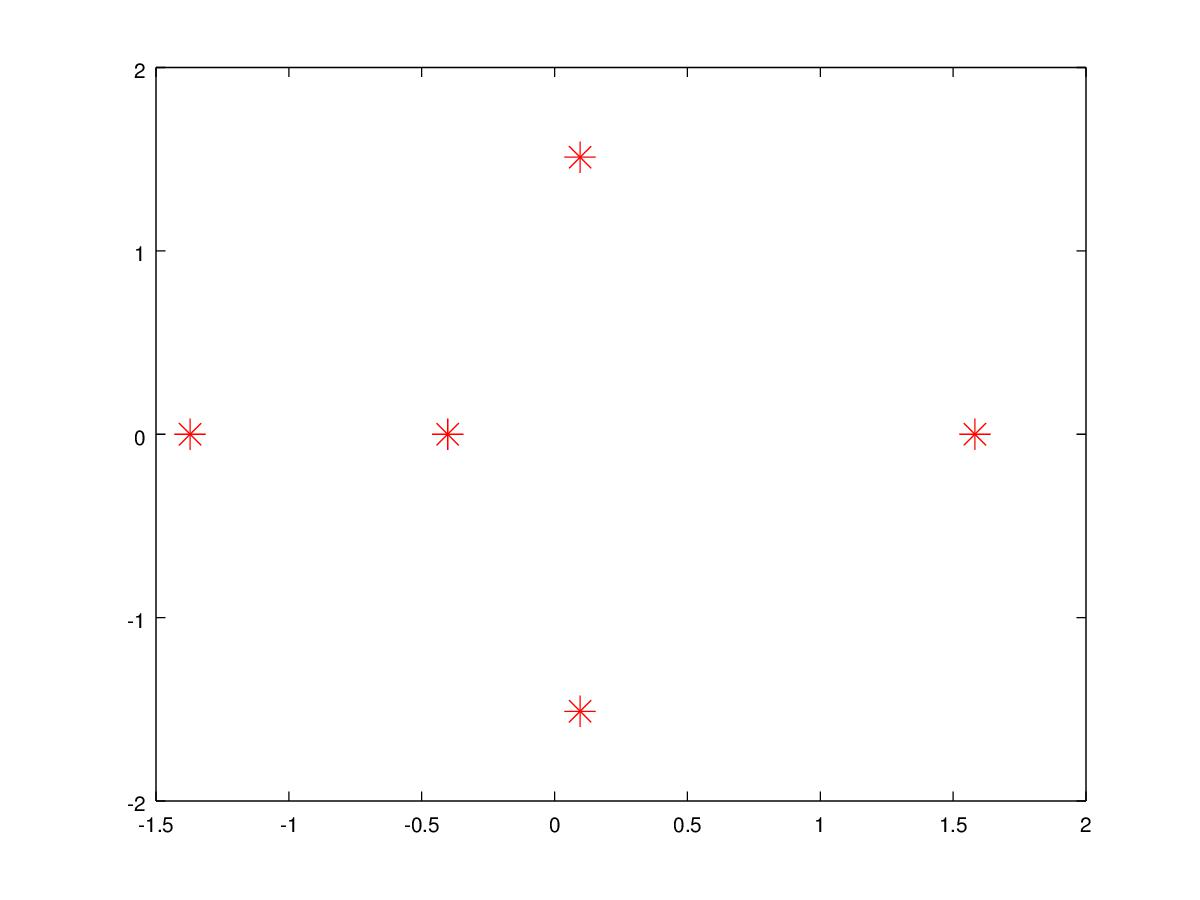
\includegraphics[width = .4\textwidth]{pic/163122zo5tmql5otmldxtf.jpg}\\
就画出这5个根在复平面的位置。}
\\
\hline
\end{tabular}
\end{center}



\kaishu
应用向量的表达,在今日可以很方便地与计算机互动来完成科研和工程中的计算和图像显
示工作。

\songti
\par
我们将从线性方程组、矩阵和线性空间,不同的角度,建立起它们的联系,让你从直观想
象中了解线性代数的内容。

	
\chapter{重修线性代数2——具象}
抽象数学概念的直观想象,是从最基本的概念开始,用已经习惯的具象,层层堆积建造而成。物理是描述现实的世界,其中的概念都经事例反复喻解,而能直观想象,任何认知的偏差,都以事实为依据来纠正。数学研究逻辑建构的抽象世界,在那里公理和定义是最终的依据,定理是可信的构件。数学为了强调逻辑推理是求证的唯一手段,防止学生误用事实和想象作依据,多数课文故意剥离抽象概念来源的事例来避免过度想象,一切通过定义和逻辑证明。这样的数学训练严谨了,学生却往往失去了有用的直观。对于数学概念和定理,直观想象因人而异使用的边际不同,都不足为凭求真,只有逻辑证明才是可靠的,但有了它能将缤纷的美色编织成图案,会指引你在这抽象世界里行走。正确的想象是由基础概念和定理累积而成的,它必须在自己头脑中通过逻辑证明的反复纠偏淬炼才有价值。

这篇用列向量和矩阵的具象,让读者回顾学过线性代数的基本概念,建立起基本图像。这里常对一个概念从不同角度做不同的解读,用心的读者可从不同的方向看到图像的不同侧面。这些都是非常基本的,大多是你已经熟悉的,但也可能有你过去忽略的视角。
\subsection{列向量和矩阵}
解析几何告诉我们,几何空间中一个点可以用它的坐标,也就是用一组数来表示。这组数也表示,从原点到这点的矢量分解在各坐标轴方向上的分量。用几何的语言来说,坐标值即是向量在坐标轴上投影的长度;向量是坐标轴单位向量的线性组合,这线性组合的系数是这些投影分量的长度;包含着这些向量的几何空间叫做向量空间。竖排着坐标值的一组数,称为列向量,或统称为向量;数组中每个数称为它的分量。

\begin{figure}[h]
	\centering
	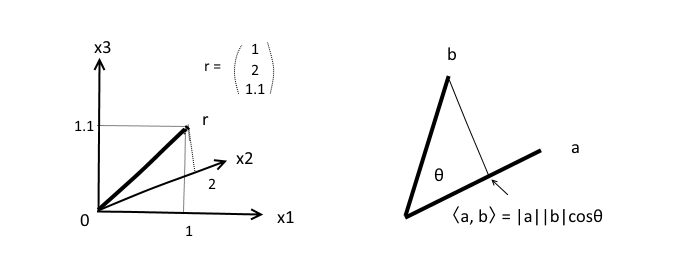
\includegraphics[width=0.7\linewidth]{pic/153404gr2s818g3sg3g1h9.png}
	\caption{向量示意图}
	\label{fig:153404gr2s818g3sg3g1h9}
\end{figure}


列向量相加等于对应的分量相加;数乘等于它乘以向量的每个分量。用$ n $个实数表示列向量的线性空间通常记为$ R^n $,其内积等于两个向量对应分量乘积后的总和,它是向量投影与投向向量长度的乘积。

用一个数组的列向量表示$ n $维线性空间中向量,以此类比三维物理空间的矢量,从三维的物理空间来推想多维的线性空间;用列向量的内积计算向量对另一个向量方向的投影长度,想象向量方向间的夹角;矩阵乘列向量,得到另一个列向量,这表示了线性算子的映射作用,不难用计算来验证这个映射是线性的。

\subsection{矩阵运算}
列向量和矩阵是线性代数中抽象概念的具体表达和运算手段。列向量可以看成仅有一列的矩阵,它的运算规则可以归纳在矩阵中来介绍。

矩阵是排列成矩形的一组数,$ m*n $矩阵是m行n列的矩阵,$ m*n $矩阵$ A=(a_{ij})_{mn} $和$ B=(b_{ij})_{mn} $相加是矩阵中相同位置的各元素相加,$ A+B=(a_{ij}+b_{ij})_{mn} $;数乘c则是c乘以矩阵A中的每一个元素$ c*A=(c*a_{ij})_{mn} $.

显然,$ m*n $矩阵相加及与数相乘仍然是$ m*n $矩阵,这叫做对线性运算封闭,即$ m*n $矩阵构成了一个线性空间。一行数组是$ 1*n $的矩阵,称为行向量;一列数组是$ m*1 $的矩阵,称为列向量,它们分别也构成了线性空间。虽然矩阵也构成线性空间,一般我们都把线性空间的元素表示成向量的形式,而用矩阵表示线性空间中的线性算子。这是在向量和算子的坐标表示中,形成的约定。

$ m*n $矩阵$ A $与$ n*k $矩阵$ D $相乘$ AD $是一个$ m*k $的矩阵$ G=AD $,其中$ G $第$ i $行第$ j $列元素定义为$ A $中第$ i $行与$ D $中第$ j $列的内积,$ G=(g_{ij})_{mk} $, $ g_{ij}= \sum_{k}^{r}a_{ir}b_{rj} $ 。

任意的矩阵相乘未必都有定义,相乘的矩阵,左边矩阵的列数必须等于右边矩阵的行数。在有定义的矩阵乘法中,显然乘法的交换律是不成立的,但多个矩阵相乘,结合律是成立的。矩阵与向量的相乘可以看作矩阵相乘的特殊情况。

乘法的交换律不成立,这在矩阵乘法算法定义下导出,也许人们不觉为奇,但是把矩阵看成是一个数学的实体,看成是线性算子的数值表示,用一个字母符号代表它,解读成一个物理变量,相乘交换律不成立,就与长期直观形成标量的代数运算相冲突。这是矩阵给经验数学之人第一个深刻的习惯改变。如果你不经意,错误的习惯会在以后继续迷惑你。量子力学奠基人之一海森堡创立矩阵力学时,曾为此苦恼过,物理学者当时难以接受也因不习惯于此。

抽象代数运算,原则上可以定义不同的矩阵乘法,例如在$ m*n $矩阵间定义同下标的元素相乘,实际上这种乘法在支持矩阵计算的软件中,叫做元素运算(Element-Wise Operations),非常有用。但是通常的矩阵乘列向量的算法定义,来自线性方程组中算子对向量作用的表达,约定的矩阵乘法定义来自复合算子的表达,这个约定乘法的设计,构建了线性代数的大厦。

\subsection{基本图像}
历史中,矩阵来自解线性方程组。往下看个具体的例子。
\begin{gather*}
	x_1+x_2=3\\
	x_1+x_2+2x_3=9\\
	x_1+2x_2+2x_3=11
\end{gather*}

这是一个线性方程组。将方程左边的系数,未知数和方程右边的数,由矩阵乘法的定义,可以写成矩阵的形式,则是:
%    \[ \begin{pmatrix} a&b\\c&d \end{pmatrix} \quad
%\begin{bmatrix} a&b\\c&d \end{bmatrix} \quad
%\begin{Bmatrix} a&b\\c&d \end{Bmatrix} \quad
%\begin{vmatrix} a&b\\c&d \end{vmatrix} \quad
%\begin{Vmatrix} a&b\\c&d \end{Vmatrix} \]

\begin{gather*}
	\begin{pmatrix} 1&1&0\\1&1&2\\1&2&2 \end{pmatrix} \begin{pmatrix} x_1\\x_2\\x_3 \end{pmatrix}=
	\begin{pmatrix}	3\\9\\11 \end{pmatrix}
\end{gather*}

分别用$ A $, \textbf{x}, \textbf{b}, 记这三个矩阵。方程用这些符号可以表示如下:

\begin{gather*}
A = \begin{pmatrix} 1&1&0\\1&1&2\\1&2&2 \end{pmatrix}, x = \begin{pmatrix} x_1\\x_2\\x_3 \end{pmatrix},b = 	\begin{pmatrix}	3\\9\\11 \end{pmatrix}, \mathbf{ Ax = b }
\end{gather*}

列向量这一组数表示线性空间中一个向量,方程式子$ \bm{ Ax=b } $ 表示矩阵$ \bm{A}$将向量$ \bm{x}$变成向量$ \bm{b}$。矩阵$ \bm{A}$的作用如同函数,实现一个映射,在空间中称为算子。这是方程、矩阵和空间中向量间最基本的关系。

矩阵乘列向量,是矩阵作为一个线性算子把这列向量映射成另一个列向量,线性方程组用计算的细节反映了这种关系。注意方程的个数未必要等于未知数的个数,即它表示成的矩阵不一定是方阵。这个方程右边的向量未必在映射算子的值域中,即解未必存在。即使它在值域中,也许它不只是一个映射的像,即解即使存在也未必是唯一的。你要从中学习惯的特殊情况中走出来。

从另一个角度,线性方程组的每一行对应着一个行向量与向量$ \bm{x} $的内积计算,方程的右边是内积的值。它表示着向量间的投影关系。

\begin{gather*}
	B_1 = \begin{pmatrix}
		1\\1\\0
	\end{pmatrix},
	B_2 = \begin{pmatrix}
		1\\1\\2
	\end{pmatrix},
	B_3 = \begin{pmatrix}
		1\\2\\2
	\end{pmatrix} \quad
	A = \begin{pmatrix}
		B_1^T\\B_2^T\\B_3^T
	\end{pmatrix},
	\begin{matrix}
		<B_1,\bm{x}>=3\\
		<B_2,\bm{x}>=9\\
		<B_3,\bm{x}>=11
	\end{matrix}
\end{gather*}

两个矩阵相乘既可以看成两个线性算子的复合,也可以看成用右边矩阵的列向量为线性组合的系数,在左边矩阵的列向量上构造出了一组的列向量,形成的另一个矩阵。

矩阵是数据的一种形式表示,其加法和乘法对应着它们元素间按它的规则运算。矩阵中的元素通常是一个数,但不限于此,它可以是任何数学实体,如矩阵、算符等,只要相应的元素间运算有意义。我们可以把矩阵分块表示和运算,这有时可以带来运算方便和解释意义。例如上面的方程可以用分块矩阵形式表示为:

\begin{gather*}
	\begin{pmatrix}
		A_1&A_2&A_3
	\end{pmatrix}
	\begin{pmatrix}
		x_1\\x_2\\x_3
	\end{pmatrix}=
	\begin{pmatrix}
		3\\9\\11
	\end{pmatrix}
	\mbox{其中} \ 
	A_1 = \begin{pmatrix}
		1\\1\\1
	\end{pmatrix},
	A_2 = \begin{pmatrix}
		1\\1\\2
	\end{pmatrix},
	A_3 = \begin{pmatrix}
		0\\2\\2
	\end{pmatrix}
\end{gather*}

它表示方程右边的向量是向量$ A_1,A_2,A_3 $的线性组合,$ x $是这线性组合系数的那组数。把矩阵看成是排成一行的一组列向量,它乘右边的列向量,相当于用右边列向量的那组数把矩阵中的列向量线性组合成一个向量。解线性方程组可以看成求这个线性组合的系数。

\begin{gather*}
	x_1 \begin{pmatrix}
		1\\1\\1
	\end{pmatrix}+
	x_2 \begin{pmatrix}
		1\\1\\2
	\end{pmatrix}+
	x_3 \begin{pmatrix}
		0\\2\\2
	\end{pmatrix}=
	\begin{pmatrix}
		3\\9\\11
	\end{pmatrix}		
\end{gather*}

\subsection{计算工具}
从计算的角度,矩阵是排列成矩形的一组数,它们打包起来用一个数学符号代表以便于批量计算和引用。其加法和数乘来自向量空间的线性,而乘法的定义则为了适用于线性组合的表示。

矩阵在计算机里是个数组,可以用这个数据结构,储存诸如一张图片的像素,一个代数方程的系数,一个季度销售的列表和实验的数据等等,在计算机语言中用一个变量来表示。它们间的运算,除了矩阵的加减乘除指数运算外,还可以定义分别对应于每个元素间的运算,例如两矩阵的元素乘法和矩阵的初等函数计算。

矩阵的计算和图像显示在今日,已经是非常基本的科研和工程的工具了。我们学习线性代数必须明白矩阵各种计算的含义和算法,通过笔算的练习掌握它。但实际工作中,如果还停留于手算,就像仍然停留在手工作业不能融入工业时代一样的落后。

在21世纪,人机互动将成为最有效率的工作方式。过去直接引用数学定理来做科研,现在直接使用计算机中的软件来协助。矩阵和图像是一种非常通用的数据表达方式,已经有许多的计算机软件提供人机互动的界面和解释程序为此工作。用于数学、统计、科学和工程中,基于矩阵计算最有名的软件是MATLAB,这是个收费商业软件。在你的手头,如果没买这个软件,建议装一个GNU免费软件Octave,它的解释程序语言与MATLAB几乎一样,而且功能非常相似。在你的学习中可以用它验证计算,熟悉它用于工作。你可在GNU官网链接中下载这个免费软件

https://www.gnu.org/software/octave/

下面是在Octave(MATLAB也一样)指令窗中,演示上述例子的线性方程组解的计算,以及用两个和三个行向量分别表示二维和三维曲线100个点的坐标来画图。用户在“$ >> $”字符开始的行,打进指令,在那行下面,指令窗口直接打印出结果,如果在指令的末尾加上分号“;”,则不打印出结果,指令行中“\%”后面是解释文字。没有用过这软件的读者,建议花几个种头读一篇入门介绍的例子,如Introductionto Octave练习一遍。熟悉这类软件的使用,就像过去学了数学有关的计算,要熟悉对数表,计算尺,计算器使用一样的重要了。
\begin{table}[htbp]
	\setlength{\abovecaptionskip}{0.cm}%%%%这个还不大清楚意思
	%\caption{Nomenclature}
	%\label{Nomenclature}
	\centering
	\setlength{\tabcolsep}{2pt}
	
\begin{tabular}{|p{170 pt}|p{170 pt}|}

	\hline
	$ >> $ A = [1 1 0;  1 1 2; 1 2 2] \%矩阵
	
	A =
	
	1    1   0
	
	1    1   2
	
	1    2   2
	
	$ >> $ b = [3;  9; 11]  \%赋值列向量 b
	
	b =
	
	3
	
	9
	
	11
	
	$ >> $ x = Ab  \%用A左除法解 Ax=b 方程
	
	x =
	
	1
	
	2
	
	3
	
	$ >> $ A*x  %验证x是方程的解
	
	ans =
	
	3
	
	9
	
	11
	
	&
	
	t 是从0到5π有100个元素的行向量
	
	$ >> $t =  linspace(0, 5*pi, 100);  
	
	$ >> $plot(t,sin(t));                   
	
	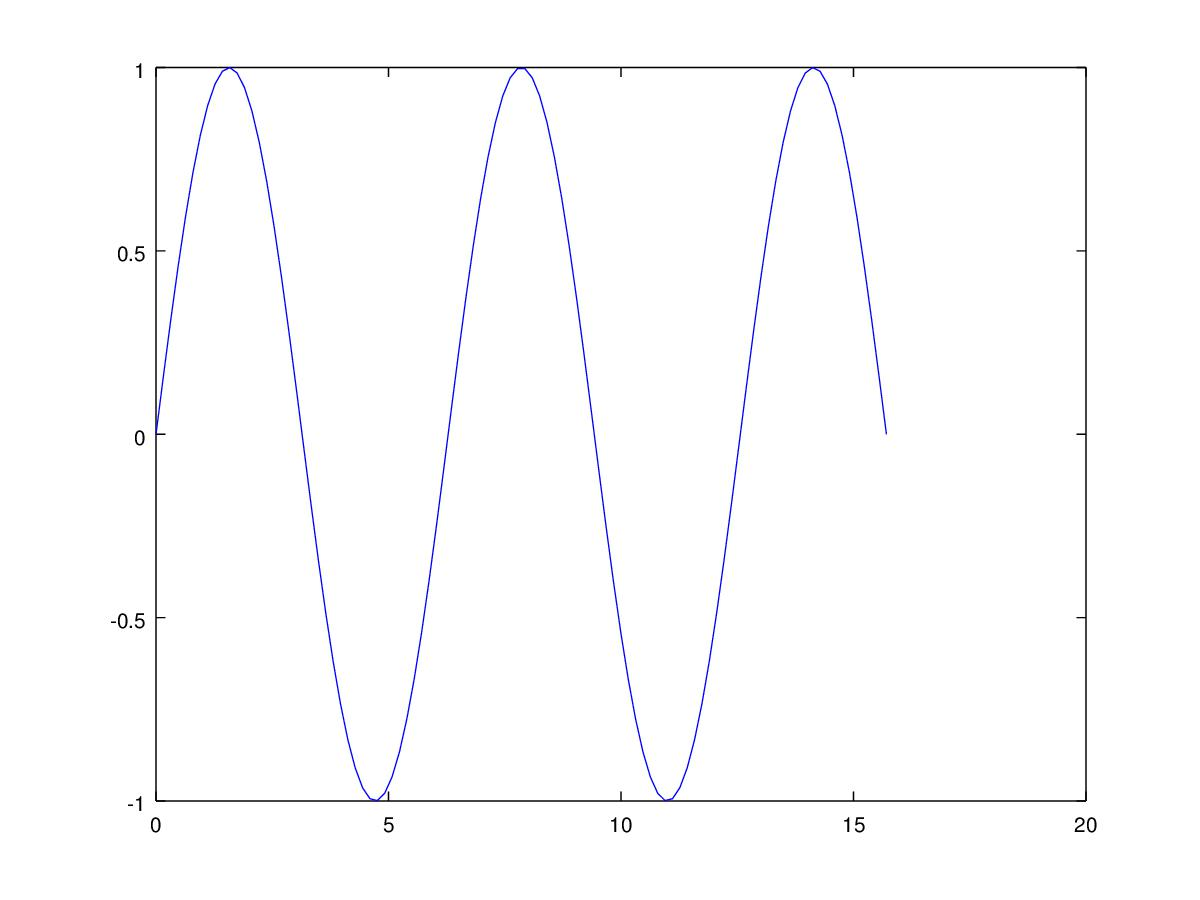
\includegraphics[width = .4\textwidth]{pic/154012hzzaaow33s7a7kst.jpg}
	
	$ >> $plot3(sin(t),cos(t),t);
	
	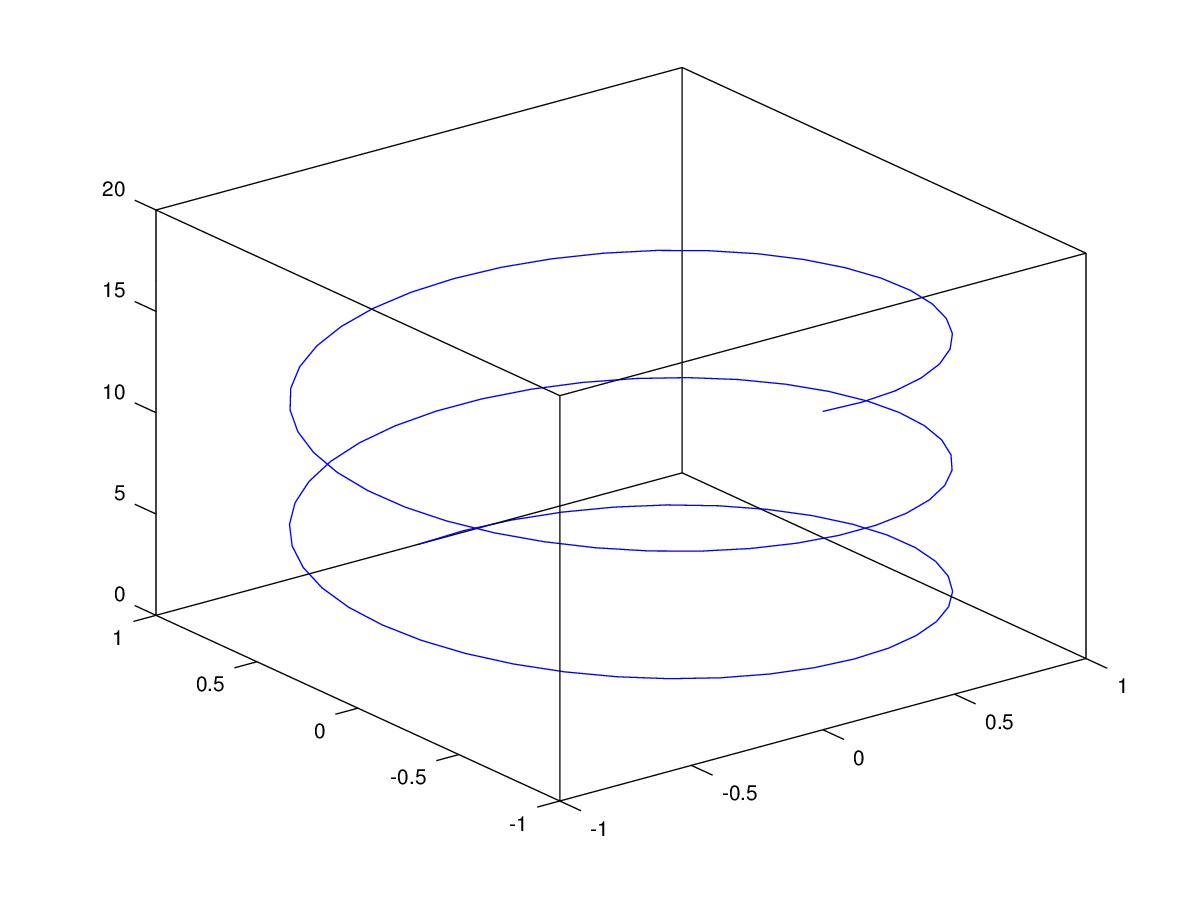
\includegraphics[width = .4\textwidth]{pic/154013uf11jfijj1nivsjn.jpg}\\
	\hline
\end{tabular}

\vspace{1.5em}%%%%%%%%%%%%%%%%%%%%缩减竖直距离%%%%%%%%%%%%%%%%%%%%%%
\end{table}
在这例子画出三维图后,用户还能用鼠标在图上旋转不同角度来观察这个空间曲线。这几个极其简单的例子,目的是给读者一个印象,用计算机可以很方便地进行矩阵计算和画图。它也是现代课程学习常用的工具。如果你还没用过,不妨现在开始熟悉它。

	
\section{重修线性代数3——抽象 }
线性代数课是从经验数学到抽象数学的一条门径。虽然不走上这抽象的台阶,绕路而行,记忆公式证明和熟练计算,也能考到高分,但学这门课,只有通过思想方法转换,上了台阶过这道门,才算不虚此行,得以进一步窥探抽象的世界。前篇的讲述是按照经验数学的思路,由具体到抽象的归纳。这篇将按公理化数学的思想,对同样的概念从抽象的定义开始,推演出它的性质。

\subsection{线性空间的定义} 

历史上的数学是无数经验的总结,曾被看作是绝对的真理。抽象过的概念,比如数和它的运算,经过千百年传承融入习惯,已变成天经地义的事实。而现代数学将形式推理,从真实世界中的关联分离出来,纯粹致力于研究抽象的概念和它蕴含的性质。这些概念只是假设的约定,也许它们源于真实世界的抽象,但我们不再关心其假设或结论真实与否,而仅仅关心逻辑的联系,将数学变成科学研究中精确表达和推理的工具。

线性代数是数学抽象的入门课。学生有时可能觉得奇怪,为什么教科书对同一个概念和定理用不同的数学理论系统,重新讲述。其实这是让你学习从不同角度看问题,让你从学习“真理”般的经验数学,转轨到“从假设到逻辑结论”方式的公理化数学。

前篇通过列向量和矩阵,由算法具体描述了向量,算子和线性空间的一些性质。这看起来像只是用个名称,命名由已知的算术运算构造出来的数学实体。你是通过对应用的了解,想象和验算来接受这被命名概念的性质。这是学物理和工程所习惯的科学思想模式。现代的数学,不是研究自然的科学,一切的概念都来自凌空而立的抽象定义,并不特定所指某一具象,这样用形式逻辑推导出来的结果,可以涵盖已经熟悉的数学实体,也能包括广泛的,符合定义但未始料及的对象。这是数学抽象的思想方式。你要从此习惯数学上对错的裁定,不借助概念所指事实的判断,除了公理、定义和逻辑之外别无所凭。

下面用数学的语言,抽象地定义线性空间和线性算子,重新走过在具象中所述的这些概念的特性。

\kaishu
集合X中的元素如果对线性运算封闭,即对于数域(有理数、实数、复数等) $\mathbb{K}$,$ x, y \in X, a, b, 1 \in \mathbb{K} \Rightarrow  x+y \in X, ax \in X $对这加法是一个交换群,对于数乘有$ a(x+y)=ax+ay, (a+b)x=ax+bx, (ab)x=a(bx),1x=x $\\
那它称为是一个\textbf{线性空间}, K 中的元素叫\textbf{标量},集合X中元素叫\textbf{向量}。线性空间又称为\textbf{向量空间}。

\textbf{线性算子}$ f $是在数域$\mathbb{K}$ 上的两个线性空间$ X,Y $中,保持向量加法和标量乘法的映射。即:\\
$ f(x+y) =f(x) + f(y), f(ax)=af(x),  \forall x, \forall y \in X, \forall a \in \mathbb{K}, \;\;f: X\rightarrow Y $\\
X到X的线性算子称为\textbf{线性变换},它是映射在同一个空间的线性算子。(注:对变换和算子术语用法,不同教科书略有不同。这系列按这里的定义。)

\songti
依照这个定义,可以验证上一篇中的数组是这里定义的向量,相同数组长度的列向量集合在它的加法和数乘运算下是个线性空间。$ m*n $矩阵是$ n $元列向量线性空间到$ m $元列向量线性空间上的线性算子,当$ m=n $时,这矩阵表示一个线性变换。

数学的对象都是抽象的,凡是符合它定义的具体东西都是它所指的对象。依此定义,只包含一个0向量元素的集合,有理数、实数以及复数的集合,分别在相应的加法和数乘定义下也都是向量空间,数乘都可看作是线性算子,这些标量作为零维和一维的向量空间和线性算子。虽然这些平凡的实现,常常被特指的介绍排斥在外,但它们符合定义,也就拥有了向量和算子概念下,逻辑推理应许的所有性质。

不难按上述的定义验证,线性空间可以包含很大的一类集合,例如,最高阶小于$ n $次的多项式的集合,$ \sqrt{2}, \sqrt{3} $
在有理数域上的线性组合,分别都构成了线性空间。线性空间还可以是无穷维的。

\kaishu
在通常的加法和数乘定义下,解析函数构成一个线性空间,求导数运算是这解析函数空间上的线性变换。除了奇点外的邻域,线性微分方程可以表示成以这线性空间上算子$ L $的形式,例如微分方程$ {y}''+a(x){y}'+b(x)y = f(x) $,可以写成算子作用的形式 $ Ly=f $,线性算子$ L(y) = {y}''+a(x){y}'+b(x)y $. 如果已知的向量$ z_i $是这线性空间的一组基向量,那么未知的向量$ y $和方程中的参数都可以表示为这些基向量的线性组合,因为算子是线性变换$  L(y) = L(c_{1}z_{1}+c_{2}z_{2}+\cdots)=c_{1}Lz_{1}+c_{2}Lz_{2}+\cdots $,对已知向量的算子作用$ c_{k}Lz_{k} $也能表示成已知向量的线性组合,这时只有线性组合的系数$ c_{k} $是待定的,代入方程求出这些待定的线性组合系数,这样解线性微分方程就变成解线性代数方程了。

解析函数在任何一点的邻域都可以用幂级数来逼近,所以幂级数在收敛的意义下包含了解析函数。特殊多项式就是上面所说的一类已知的基向量。它们虽然有无穷多个,但存在着递推关系的有限个线性组合是可计算的。这便是用它来求解线性微分方程的理论基础。

除了幂级数外还有许多函数类都能构成所在线性空间中的一组基向量,用来逼近方程的参数和它的解。物理中许多的微分方程,例如数理方程等都是线性的,对各类线性微分方程用合适的函数类可以较方便得出结果。尽管物理学家赋予它们各种物理解释,如波和粒子,但其数学功能仅仅是个基向量。在计算机时代之前,200多年间许多数学家和物理学家,都在努力应用函数级数来解线性微分方程。

\songti

长度为2和3的列向量集合不构成线性空间,因为它们对通常列向量的加法运算不封闭,但如果我们在定义列向量加法时,将较短的列向量计算时用0补足长度,它们在这定义下构成了线性空间。所以,抽象的数学概念必须通过直接对定义的检验来确定。数学上的代数概念总是与集合中元素运算的定义相关,数学空间不仅仅指它的基础集合,而且必须符合它上面运算的定义和封闭性。

在学习线性代数中要开始了解到:从定义出发非常不同的数学对象,可以从属于同一数学概念;而同一个数学实体在不同的运算定义下,也可以分属不同的数学概念。要开始习惯不再从整数、有理数、实数、复数、函数层层叠高复合构造中来理解这些数学实体,而是从抽象约束的视角对数学实体做概念上的判定,这是从一种普遍化抽象代数的角度来研究数学问题。矩阵的乘法,让我们开始从过去习惯的交换律中挣脱出来,感受到乘法的运算未必都可交换顺序的。

上大学数学课容易发生两种偏差,一是仍然沿着经验和学物理的思想模式来学数学,这样虽然在计算应用上没有问题,积弊是失去严谨的修炼和抽象的视野。以后学习较深数学时,会感到吃力,这是因为错过了该走的台阶。重修时,对每个概念的定义,要用举例和反例来对照理解。这些已在课本中的逻辑证明,我们就不在这系列中重复了。

另一偏差是,谨守从定义开始逻辑证明的路径,致力于记忆这个过程和结论。殊不知这个严谨的逻辑推理,仅仅是数学严谨的修炼,是构建可靠图像的必经途径,它是串起珍珠的丝线。没有消化变成自己头脑中的图像,是买椟还珠,考试过后就还给了老师,十分可惜。丰富的直观感觉依赖于从基础开始,层层构筑起来的图像。这要像学习物理一样,对每个概念都能从性质和定理看到内在关系。这个系列主要引领读者走过这条路。请注意,如果你不能确信想象的正确性,你就必须用公式推导来验证,重走错过路。

严谨的数学除了定义和逻辑一切都不足为凭,但为了能够理解抽象的定义,在头脑中必须与已有形象建立起联系,从而形成长期记忆,并能联想应用,我们必须有一个具体的形象。将这里的抽象定义与上一篇的具象联系起来,我们可以想象线性空间的图像是几何中的三维空间,向量是从原点出发指向空间中某一点的有向线段,线性变换可以看成对空间中的几何图像对原点的旋转、翻转、剪切和伸缩。这个系列在帮助读者建立起几何图像时,都用实数作为数域为例来想象,读者可以参照定义对有理数和复数域自行修补图像。

数学的对象是抽象的形式的,物理的对象是具体的真实的。数学同一的概念可以用来表示不同的物理对象,而物理的对象可以用不同的数学工具来处理。学习数学与物理不同之处在于,数学需要牢记的是定义,在这里要记忆线性空间、线性算子和线性变换的数学定义,并随时用它们来检验例子和想象中的对象,在不断检验过程中就会记住了定义的内涵,构造反例来约束错误的联想。你必须学会通过具象中想象定义和可能的结果,有能力在不确定时用逻辑从定义出发严格地证明,纠正错误的想象加深正确的印象,在头脑中建立起抽象世界的图像。

\subsection{内积}
一组向量,如果其中一个能表达成其他的线性组合,则说它们是\textbf{线性相关}的,否则是\textbf{线性无关}的。如果线性空间中最大线性无关组的向量个数是$ n $,则称它是\textbf{n维线性空间}。线性空间中任何的向量都可以表示为一组线性无关向量的线性组合,这组向量称为线性空间的\textbf{基}。线性空间的基不是唯一的,但组中向量的个数都等于空间的维数。任何一组$ n $个线性无关向量都可以是$ n $维线性空间中的基。

线性空间的定义仅仅关注集合元素间线性运算的性质。它只触及向量间“代数的”性质,两个向量之间除了它们是否有数乘关系之外别无其他,没有夹角、距离、长度等等几何的性质,这与列向量和矩阵的具象所拥有的丰富图像相差甚远。

为此引入两个向量间关系的内积概念。让拥有它的数学空间具有更丰富的内容。

\kaishu

设$ X $是数域$ \mathbb{K} $(通常是实数或复数)上的线性空间,定义映射$ \left\langle x,y \right \rangle :X\times X\rightarrow \mathbb{K} $,称为$ X $上的\textbf{内积},如果它满足下列性质:$ \forall x,y,z \in X, \forall a,b \in \mathbb{K} $有\\
正定性:$ \left\langle x,x\right \rangle \ge 0, \left \langle x,x \right \rangle = 0\Leftrightarrow x=0 $\\
共轭对称性:$ \left\langle x,y \right \rangle = \overline{\left \langle y,x \right \rangle} $\\
对第一变量的线性:$ \left\langle ax+by,z \right \rangle = a\left \langle x,z \right \rangle + b \left\langle y,z \right \rangle $\\
赋以内积性质的线性空间称为\textbf{内积空间}。(注:有的教材的定义是对第二变量线性。)

定义范数$ \Vert x \Vert = \sqrt{\left \langle x,x \right\rangle} $
,称为向量x的长度,如果按其导出的距离是个完备的距离空间,则称它是\textbf{希尔伯特(Hilbert)空间}。

\songti

有时,我们把向量$ x $和$ y $的内积表示为$ x \cdot y $,称内积为点积。

依此定义,由列向量构成的线性空间,以共轭分量乘积和的运算定义构成了内积空间,同时也是个希尔伯特空间。只不过有限维空间具有平凡的完备性,希尔伯特空间一般特指是无穷维的情况。

两个向量内积为0,称为它们是\textbf{正交}的,长度为1的向量称为\textbf{单位向量}。两个单位向量的内积可以看作它们间的投影值,即定义为\textbf{夹角}的余弦。向量在一组单位正交基的坐标,是它对每个基向量方向的投影值。线性空间的两组基之间对应着一个满秩的线性变换,向量对两组基的坐标之间对应着一个满秩的正方矩阵。读者花点时间,用三维空间中向量的夹角、投影和解析几何中的图像,想象一下向量对一组基的坐标值,及线性算子的具体矩阵表示,建立起这个直观想象对学习线性代数十分重要。

与任何概念的数学定义一样,这里内积的定义是抽象的,满足它的具体实现可以有很多。例如,列向量的内积可以是通常定义那样,也可以是其他,比如说在那个对应分量乘积和的计算中,对第$ i $个分量乘上一个正数$ a_i $,不难验证这也符合内积的定义。这体现的是一个非各向同性的实现。

从抽象的线性代数角度来看待不同形式的数学内容,可以让你很直观地看到本质。下面是个例子。

\kaishu

柯西-施瓦茨不等式的内积形式$ |\left \langle x,y \right \rangle |\le \|x\|\|y\| $,这在几何上十分直观,无非是向量在任何方向的投影长度不大于它本身,或余弦的绝对值小等于1等等。当然,任何直观要确认它成立,必须用严格的逻辑来证实。证明的思路就是参照直观的图像,构造一个向量$ z $,它与$ x $正交,即$ \langle z, x\rangle = 0 $,且与$ y $投影到$ x $的向量相加等于$ y $,即$ z=y - \langle y, x \rangle x/\|x\|^2 $,用内积定义里的正定性$ \|z\| \ge 0 $,不难用纯粹的代数形式推演,得出内积与这两个向量间的关系。

在以前的数学学习中,读者可能见过不同形式的柯西-施瓦茨不等式和它们的证明。

\begin{gather*}
	|\sum_{i=1}^n x_iy_i|^2 \le (\sum_{i=1}^n x_i^2)(\sum_{i=1}^n y_i^2)
\end{gather*}
\begin{gather*}
	|\int f^*(x)g(x)dx|^2 \le \int |f(x)|^2 dx  \int |g(x)|^2 dx
\end{gather*}

其实对于上面两个不等式,在$ \mathbb{R}^n $
和$ L_2 $的线性空间中分别定义它们的内积为等式左边绝对值里的式子,直接从内积形式的不等式中就可以得出这些等式,对于复数和矩阵形式的相应的不等式也是如此的简单。

\songti

	\section{重修线性代数4——表达} 
抽象的线性空间涵盖许多不同的数学实体,而它们可以表达成列向量和矩阵来计算。将抽象空间中的运算一一对应到一个具体空间中来研究,这是学习抽象方法的一个重要入口。习惯了它,在学习抽象代数时,你就能自然地欣赏同构,同态和商空间运用的美妙。

\subsection{基与坐标}

线性代数课程主要在讲矩阵的运算。这是为什么?列向量和矩阵仅仅是抽象线性空间中向量和线性算子的一个具体实现,满足抽象定义的具体数学实体有无数种,线性空间和算子的许多证明都直接在矩阵上讲,而不是根据一般的抽象定义来证明,这样的结论会具有普遍性,能适用于其他吗?

这里的原因,一是作为抽象数学的入门课,线性代数课从列向量和矩阵开始的学习内容,提供了一个从直观的构造主义传统数学,到抽象的形式主义公理化现代数学思想方法的过渡。另一是,列向量和矩阵可以看成各种向量和线性算子的表达,它们之间建立起的一一对应关系,在线性运算中也保持,在线性代数的结构上是等价的,所以相关结论也适用于其他。

如果一个线性空间X里线性无关向量组里最多有n个向量,n是有限的,那么它称为\textbf{n维线性空间}。记为$ dim(X)=n $.  例如长度为n数组的线性空间是n维的。最高阶小于n的多项式空间是n维的。

两个数学空间X,Y,如果它们间的元素存在着一个一一满映射σ,对抽象空间中的运算φ有 % MathType!MTEF!2!1!+-
% feaahqart1ev3aaatCvAUfeBSjuyZL2yd9gzLbvyNv2CaerbuLwBLn
% hiov2DGi1BTfMBaeXatLxBI9gBaerbd9wDYLwzYbItLDharqqtubsr
% 4rNCHbWexLMBbXgBd9gzLbvyNv2CaeHbl7mZLdGeaGqiVu0Je9sqqr
% pepC0xbbL8F4rqqrFfpeea0xe9Lq-Jc9vqaqpepm0xbba9pwe9Q8fs
% 0-yqaqpepae9pg0FirpepeKkFr0xfr-xfr-xb9adbaqaaeGaciGaai
% aabeqaamaabaabauaakeaacaqGGaGaeqy1dyMaaiikaiabeo8aZjaa
% dIhacaGGSaGaeq4WdmNaamyEaiaacMcaaaa!4913!
\[{\rm{ }}\phi (\sigma x,\sigma y)\] ,即其一空间中的运算完全对应于在另一个空间中的运算,则称为它们是\textbf{同构}的。如果忽略同构对象的属性和运算的具体定义,就结构而言,同构的对象是等价的。相同维数线性空间之间的满秩线性算子,即是一个能够保持线性运算的一一满映射,所以相同维数的线性空间都是同构的。

同构意味空间的数学结构是一样的,在抽象代数学习中,可以用其中一个简单熟悉的数学实体作为代表来作研究。对于线性空间,列向量和矩阵就是这个的代表,有限维线性空间的计算和性质可以通过它们的计算来实现。

向量和线性算子都能表示成数域上的列向量和矩阵。这列向量在有限维的线性空间是有限的数组,在无穷维的空间则是无穷级数中的系数或积分中的加权函数项。下面介绍其映射关系。

取n维线性空间X中一组n个线性无关的向量,$ {e_1,e_2,\cdots,e_n} $,称为一组基,按最大线性无关组的定义,X中任何向量都可以分解为基向量的线性组合,

\begin{gather*}
	{r} = r_1{e_1} + r_2{e_2}+ \cdots + r_n{e_n} =\begin{pmatrix} {e_1} &{e_2}  &\dots  & {e_n}\end{pmatrix} \begin{pmatrix}r_1 \\ r_2 \\ \vdots \\r_n \end{pmatrix}
\end{gather*}

向量$ r $对这组基分解的系数,称为向量在这组基下的坐标,它们是一组数,把它排成一列按矩阵的形式运算,表示为上面的列向量$ (r_i)_n $. 列向量线性空间$ \mathbb{R}^n $的基,是$ n $个只有一个分量为1,其余都为0的数组集合。把列向量看成坐标的数组,在列向量作为线性空间X中向量坐标表示的映射中,$ X $的基向量$ ei $对应着$ \mathbb{R}^n $的,只有第i分量是1的基向量。

给定一组基下的线性表示,n维线性空间X中的向量与数域上n阶的列向量建立起一个一一对应的满映射。不难证明这种对应关系,对向量的加法和数乘也保持。相同数域上的相同维数的线性空间都是对线性运算同构的。这意味着n维线性空间中的线性运算,都可以通过映射对应到对列向量的运算。

显然在不同的基上,同一个向量的坐标表示是不同的。

\kaishu

例如所有的小于5次的多项式构成一个5维线性空间,$ 1, x, x^2, x^3,  x^4 $, 是一组基,所有小于5次的多项式都可以表示成它们的线性组合。式子$ x+1, x-1, (x-1)^2,(x-1)^3,(x-1)^4 $也是一组基,这空间里的多项式也都可以表示为它们的线性组合。

\songti

设$ \alpha $是n维线性空间X到m维线性空间Y的一个线性算子,$ {e_1,e_2,\cdots,e_n} $ 和
  $ {g_1,g_2,\cdots,g_m} $ 分别是X和Y上的一组基,$ \alpha e_j $是Y上的一个向量,可以表示为 $ a_{1_{j}}g_1+a_{2_{j}}g_2,+\cdots+a_{m_j}g_m $,所以对X上的任意向量r,我们有

\begin{gather*}
	\alpha\textbf{r}=\alpha \sum_{j=1}^n r_j \textbf{e}_j = \sum_{j=1}^n r_j \alpha \textbf{e}_j = \sum_{j=1}^n r_j \sum_{i=1}^m a_{ij}\textbf{g}_i = \sum_{i=1}^m( \sum_{j=1}^n a_{ij} r_j)\textbf{g}_i	
\end{gather*}

将等式右边表示成矩阵形式就是:

\begin{gather*}
	\begin{pmatrix}\textbf{g}_1,& \textbf{g}_2,& \cdots,& \textbf{g}_m \end{pmatrix}\begin{pmatrix} a_{1,1}& a_{1,2}&\cdots& a_{1,n} \\ a_{2,1}& a_{2,2}&\cdots& a_{2,n} \\ \vdots& \vdots & \ &\vdots \\ \vdots& \vdots & \ &\vdots  \\a_{m,1}& a_{m,2} &\cdots& a_{m,n} \end{pmatrix} \begin{pmatrix}r_1 \\r_2 \\ \vdots \\r_n \end{pmatrix}
\end{gather*}

n维到m维线性空间上的线性算子$ \alpha $,在给定的基下表示为一个m*n数域上的矩阵A,矩阵中n个列向量,分别对应于$ \alpha $将n维空间每个基向量,映射到m维空间上向量的坐标表示。这个线性算子对向量r的作用所得向量的坐标列向量,等于矩阵A乘以r的坐标列向量。类似的,可以证明复合线性算子的矩阵表示,等于它们表示矩阵相乘所得的矩阵。

同一个线性空间上的线性算子对加法和数乘构成一个线性空间,它与算子的矩阵表示构成的线性空间,对线性运算和乘法运算都是同构的。所以通过基形成的对应关系,线性空间的向量和线性算子的运算都可以通过列向量和矩阵的运算来表示。

\kaishu

函数求导是一个线性运算,它也是在那个小于5次的多项式线性空间上的一个线性变换,在 ,$ 1, x, x^2, x^3,  x^4 $,的基下,它可以表示为一个矩阵D,多项式$ x^4+2x^3-3x^2+x+12 $在这组基下表示为向量r,对这多项式求导得到$ 4x^3+6x^2-6x+1 $,也可以从下面矩阵运算中体现。

\begin{gather*}
	D=\begin{pmatrix}0&0&0&0&0\\4&0&0&0&0\\0&3&0&0&0\\0&0&2&0&0\\0&0&0&1&0 \end{pmatrix},r=\begin{pmatrix}1\\2\\-3\\1\\12\end{pmatrix},  Dr=\begin{pmatrix}0\\4\\6\\-6\\1\end{pmatrix}
\end{gather*}

请在$ x+1, x-1, (x-1)^2,(x-1)^3,(x-1)^4 $这组基下写出这例子中的矩阵、向量并验算求导的答案。问这矩阵的秩是多少,给出一个零空间中的向量。

\songti

在你头脑的图像中,向量、基向量、线性算子所指的,是有向线段、坐标轴、多项式、函数等等数学世界符合抽象定义规范的东西。而这些向量和线性算子,对应着在基坐标的列向量和矩阵,是它们在数值世界上的影像。在不需要区分时,人们经常直接用列向量和矩阵代表所对应的向量和线性算子。在不同的基下,同一个向量和线性算子有不同的列向量和矩阵表示,这就像我们用不同的角度来描述同一个物体一样。它们之间对应着一个坐标变换。

\subsection{坐标变换}

满映射的线性变换,称为是满秩的。满秩线性变换矩阵中的列向量组是线性无关的,其矩阵的行列式不等于零。当表达线性空间X从一组基 $ {e_1,e_2,\cdots,e_n} $ 换成另外一组新的基 $ {g_1,g_2,\cdots,g_n} $ 时,同一个向量r对应于这旧的基上的坐标列向量 $ (r_i)_n $ 也相应变化成新的坐标列向量 $ (h_i)_n $ . 

记n维线性空间X中两组基间的线性变换为T,它把旧的基$ {e_1,e_2,\cdots,e_n} $变换成新的基$ {g_1,g_2,\cdots,g_n} g_i = \mathbb{T}e_i, i=1,2,\cdots,n$ ,这可以表示成一个满秩的n阶方阵$ \mathbb{T} $,其中的列向量对应着新的基向量在旧的基下的坐标。

\begin{gather*}
	\begin{pmatrix}{g}_1& {g}_2& \cdots & {g}_n \end{pmatrix} = \begin{pmatrix} \mathbb{T}\textbf{e}_1& \mathbb{T}{e}_2& \cdots & \mathbb{T}{e}_n \end{pmatrix} =\begin{pmatrix} {e_1} &{e_2}  &\dots  & {e_n}\end{pmatrix}T
\end{gather*}

它将X中向量r在新的基下坐标的变换成旧的基下的坐标。

\begin{gather*}
	{r}= \begin{pmatrix} {e_1} &{e_2}  &\dots  & {e_n}\end{pmatrix} \begin{pmatrix}r_1 \\ r_2 \\ \vdots \\r_n \end{pmatrix} = \begin{pmatrix}{g}_1 & \textbf{g}_2& \cdots &\textbf{g}_m \end{pmatrix}\begin{pmatrix}h_1 \\ h_2 \\ \vdots \\h_n \end{pmatrix}=\\
	\begin{pmatrix} {e_1} &{e_2}  &\dots  & {e_n}\end{pmatrix} T \begin{pmatrix} h_1 \\ h_2 \\ \vdots \\h_n \end{pmatrix} \Rightarrow \begin{pmatrix}r_1 \\ r_2 \\ \vdots \\r_n \end{pmatrix} = T\begin{pmatrix}h_1 \\ h_2 \\ \vdots \\h_n \end{pmatrix}
\end{gather*}

记 $ T_i $ 是新的基向量 $ g_i $ 在旧的基 $ {e_1,e_2,\cdots,e_n} $ 上坐标的列向量,矩阵 $ T=(T_1, T_2,\cdots,T_n) $ ,它是由新的基向量在旧的基地上坐标列向量排成一行的矩阵。向量在旧的基上坐标的列向量,是新的基上坐标的列向量,对新旧基表示的列向量$ {T_1, T_2,\cdots,T_n} $的线性组合系数。

不难看出对应于不同基坐标的列向量之间是个满秩的线性变换。$ T^{-1} = (F_1,F_2, \cdots, F_n) $,其中 $ (F_i)_n $ 是旧的基向量 $ e_i $ 在新的基上坐标的列向量。满秩的方阵也代表着一个坐标变换。


\subsection{坐标变换中的矩阵表示}

线性算子是从一个线性空间到另一个线性空间的映射。算子$ \alpha $的作用将$  $n维线性空间$ X $中的向量,变成$ m $维线性空间$ Y $中的向量,在给定这两个空间的基上,它表示为一个$ m*n $矩阵$ A $。两个线性空间的基是各自独立的,可以各自分别更换。继续沿着向量坐标变换的思路可以看出,在两个空间基的更换中,如果$ X $中坐标变换的矩阵是$ V $,在$ Y $中是$ U $,在新的两个基上,$ \alpha $的矩阵表示是$ U^{-1}AV $.

通过满秩变换P和Q,把一个矩阵A变为另一个矩阵B=PAQ,称矩阵A和B是\textbf{等价}的。P和Q都是满秩的方阵,$ P^{-1} $和Q分别可以看成是算子输入和输出空间的坐标变换,等阶的矩阵可以看成是同一个线性算子在不同坐标系下的表示。

线性变换是线性空间到自身的映射。变换的输入和输出在同一个空间。在给定的基上,它的作用表示为一个方阵A。基的更换不仅影响着变换作用输入的向量表示,同样影响了输出的向量表示,所以当新旧基间坐标变换为T,在新的基上,矩阵的表示将是$ T^{-1}AT $,它与旧基上的A是相似的矩阵。

任何满秩的方阵T都对应着一个坐标变换,矩阵$ B=T^{-1}AT $,称A和B是\textbf{相似}的,说明它们可以通过坐标变换来相等。相似的矩阵是同一个线性变换在不同基上的表示。

对于一个方阵A,它是既可以表示一个线性变换,也可以是一个线性算子,当它代表一个线性算子时,输入X和输出Y是相同维数的不同空间。它们的坐标变换是分别独立的。

\subsection{标准正交基}

向量对一组基的线性组合分解是唯一的,这直接可以从基的线性无关性来证明。但这只是说明这个线性空间与相同维数列向量的欧几里德空间是一一对应,而且是同构的。这并不意味着这种映射是唯一的,即不意味着对应的坐标是确定的。到目前为止,我们都不确定向量在基上的坐标,因为这涉及到向量与基向量之间的关系。引入两个向量间关系的内积概念,将让这个坐标映射清晰起来。

假设向量表达成基向量的线性组合的式子,用基向量对这表达式两边取内积,得到一个以坐标为未知数的线性方程组,它的解便确定了向量在这基上的坐标。

如果基中的向量长度都为1,并且相互正交,它则称为\textbf{标准正交基}。向量在标准正交基上的坐标等于向量在那个基向量上的投影,即它与基向量的内积。如果两组基都是标准正交基,那么它们间的变换T便是一个正交阵(酉阵对于复数域),它的转置(共轭转置对于复数域)便是它的逆,把向量新坐标变成它旧的坐标。

列向量只有在作为标准正交基坐标上的向量表示时,它的内积才等于所表示向量的内积。在一般情况下,基向量的内积构成一个正定矩阵 $ E = ( e_1, e_2, \cdots$  $, e_n )$$  T $ $ \cdot(e_1,e_2,\cdots,e_n) $ ,
向量$ x, y $的内积等于它们在这基上坐标表示列向量 $ (x_i)$ ,  $(y_i) $ 与它的乘积 $(\bar{x}_i)^TE(y_i) $ . 所以,列向量作为内积空间向量的坐标表示时,它是在标准正交基上的表示。用标准正交基上的向量坐标表示,内积等于一个列向量共轭转置与另一个列向量的乘积。这样列向量所在的坐标空间与内积空间才是同构的。

前面说,满秩的线性算子建立起相同维数的线性空间的同构关系,这只是对线性运算而言。但这并不足以保证对应的内积运算也相等。内积空间还包含着内积的运算,能保持内积空间同构的线性算子,是正交阵(酉阵对于复数域)。从几何直观来看,在线性算子作用下保持向量的长度和夹角不变(即内积不变),这个作用只能是旋转和翻转的组合。

这一小节陈述了着线性空间坐标变换关系的直观图像。如果读者不能在脑海中清晰地看到,建议花点时间,在代数表达式推演的帮助下来消化理解。有了对同一个向量和线性变换,在不同基下列向量和矩阵坐标变换的直观理解,将会比较容易看清抽象的概念与具体的数值表示间的关系。
		\chapter{重修线性代数5——空间}
	把线性空间分解成为对其运算封闭的子空间,了解子空间的直和,正交子空间,以及由算子生成的零空间和像空间,这对分析算子,简化计算以及了解结构都是一把犀利的解剖刀。
	
\subsection{子空间}
	
	线性空间是对线性运算封闭的集合。线性空间中的一个子集,如果也对线性运算封闭,即它里面任何几个向量经过线性组合后仍在这子集中,则称为\textbf{线性子空间},在没有歧义的情况简称为\textbf{子空间}。很明显,线性空间本身以及单个零向量都是平凡的子空间。一切子空间都包含着零向量。不要把子空间想象成空间中一个有边缘的几何体,子空间中任何向量的数乘,即任意的延伸都在这子空间里。高于一维的线性空间有无数不同的子空间。在三维空间中,一维的子空间是过原点的一条直线,二维子空间是过原点的一个平面,你以此来推想高维的子空间。
	
	一组向量的线性组合构成了一个子空间,称为这组向量张成的子空间。这子空间的维数,等于这组向量中线性无关向量的个数。一组线性无关的向量,意味着其中任何一个向量都不能在其它几个张成的子空间里,这就像平行六面体的三条棱边不在任何两边确定的平面里。
	
	子空间的交集仍是一个子空间,它们的并集一般则不是,但可用里面向量的线性组合扩充成一个子空间。任取一组向量,它们所有线性组合的集合是个子空间,称为这组向量张成的线性子空间。显然任何一个向量都可以张成一维子空间,k个线性无关的向量张成k维子空间,线性空间中的基张成了整个线性空间。
	
	线性空间中的几个子空间,如果它们相互间除了零向量外没有交集,它们张成的空间,称为这些子空间的直和。直和空间中的向量,都可以用这几个子空间中各有一个向量之和组成,这种分解是唯一的。直和空间里向量运算,等于它分别在子空间里的运算之和。
	
	\kaishu
	
	例如:$ a\begin{pmatrix}1\\2\end{pmatrix},\; b\begin{pmatrix}0\\ 1\end{pmatrix}, \;\; \forall  a,b \in \mathbb{R} $分别都是 $ \mathbb{R}^2 $ 的一维子空间,$ \mathbb{R}^2 $ 是它们的直和。
	
	\songti
	
	分别来自两个子空间中的向量,如果它们的内积都为零,则称这两个子空间是\textbf{正交的}。它们张成的空间是它们的直和。不是全空间或单个零向量的子空间称为\textbf{真子空间}。与真子空间正交的向量构成与它正交的子空间,它们的直和是全空间。
	
	\kaishu
	
	矩阵   $ A=\begin{pmatrix} 1&1&0 \\1&0 &1\end{pmatrix} $  的两个行向量张成  $ \mathbb{R}^3 $ 的二维子空间。方程 $ Ax=0 $ 的所有的解 $ x= a\begin{pmatrix}1&-1&-1 \end{pmatrix}^T,a\in \mathbb{R} $  构成 $ \mathbb{R}^3 $的一维子空间。不难验证$ A $的行向量张成的空间和这方程的解空间是正交的,它们的直和是  $ \mathbb{R}^3 $ 。
	
	\songti
	
	假设线性空间X是子空间W和V的直和,因为向量对子空间直和的分解是唯一的, X中每个向量都对应着子空间W中的一个向量,这个映射称为X对W子空间的\textbf{投影}。空间X中的向量线性运算与它们在W子空间中的投影也保持这种对应,这个性质称为线性空间X与它的子空间W是同态的。\textbf{同态}是在两个代数结构中保持运算不变的映射,对子空间的投影映射是一个同态映射。以前介绍的“同构”,则要求这种映射还是一一满映射。同态映射定义了一种等价关系,它把等价的元素映成同一个像元素,而令其等价的称为同态映射的\textbf{核}。子空间V是X投影到W映射的核,它的投影是零向量,如果X中任何两个向量之差在V中,它们对投影映射则是等价的,投影到W中同一个向量。由此可以进一步学习泛代数的概念,定义在等价关系下的\textbf{商空间},以及商空间与映射像同构关系的基本定理。
	
	\subsection{算子的零空间和像空间}
	
	线性算子保持两个空间的线性运算不变,所以它是一个同态映射。线性算子$  f:X \to Y $ 它的核 $ Ker(f)  $和像$  Im(f) $  定义如下:
	\begin{gather*}
		Ker(f) = \{ x\in X | f(x)= 0 \} ,Im (f) = \{f (x)| x \in X\}  
	\end{gather*}

	$ Ker(f)  $是$  X  $中被$ f $映射为0的向量构成的子空间,也称为算子的零空间。$ X $中两个向量之差如果在零空间中,它可以被线性算子看成是等价的,它们被映到$ Y $中的同一个向量。
	
	而$ Im(f)  $是 $ X $中所有向量被$ f $映射到$ Y $的像构成的子空间,也称为算子的值域。对这些子空间的维数有\textbf{秩-零度定理}:  $ dim(Ker(f))+dim (Im(f))=dim(X) $,它是线性代数的一个基本定理。
	
	\begin{figure}[h]
		\centering
		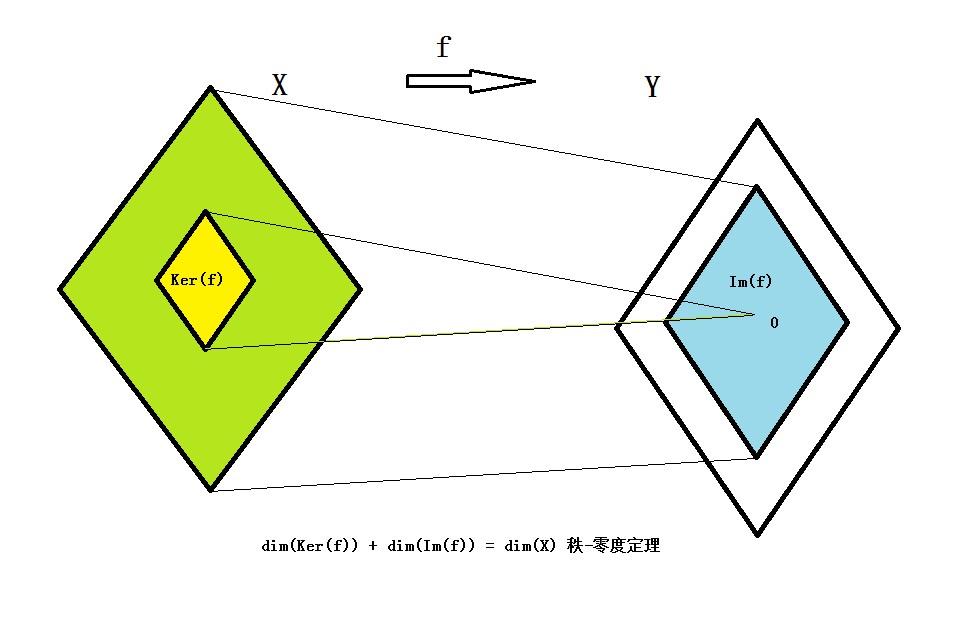
\includegraphics[width=0.7\linewidth]{pic/160449rx8lvzcxlgan88va.png}
		\caption{秩-零度定理}
		\label{fig:160449rx8lvzcxlgan88va}
	\end{figure}
	
	
	维数$  dim(Im(f))  $叫做线性算子f的\textbf{秩},记为 $ rank f $,$ dim(Ker(f)) $叫做线性算子$ f $的\textbf{零度},记为$ nullity f $。满映射的线性算子称为是\textbf{满秩}的,满秩的线性算子的零度为0. 
	
	这个定理似乎很抽象,下面我们从矩阵和方程的角度来看它。
	
	线性算子$ f $将$ X $中的向量$ x $映成$ Y $中的向量,如果存在着$ Y $上的一个线性算子$ f* $,它将$ Y $中的向量$ y $映成$ X $中的向量,使得内积$ \left\langle y, f(x)\right\rangle = \left\langle f*(y), x\right\rangle $,算子$ f* $称为$ f $的\textbf{共轭算子}。不难证明,在实数域算子的矩阵表示中,$ A $的共轭算子是它的转置矩阵$ A^T $(在复数域上是A的共轭转置矩阵$ A* $,为直观起见,我们只介绍实数域的情况,读者自行修正复数域上表示。)
	
	将线性算子$ f $表示为矩阵$ A $,$ A $的列向量张成的子空间称为$ A $的\textbf{列空间},它是算子A的像空间。$ Ax=0 $解构成的子空间称为$ A $的\textbf{右零空间},它是算子$ A $的零空间。
	
	$ A $的行向量张成的子空间称为$ A $的\textbf{行空间},它是共轭算子的列空间。共轭算子$ A^T $的零空间称为$ A $的\textbf{左零空间}。	
	
	齐次线性方程$ Ax=0 $的解构成$ A $的零空间,这方程式说明矩阵的行向量与方程解列向量的内积为零。所以,矩阵的行空间与右零空间总是正交的,它们的直和是矩阵作为线性算子定义域的线性空间。将矩阵转置,对$ A^T $也有相同的结论,即矩阵$ A $的列空间与左零空间也总是正交的,它们的直和是矩阵作为线性算子值域所在的线性空间。矩阵把它的定义域空间X分解为正交的右零空间和行空间的直和,把值域空间分解为正交的左零空间和列空间的直和。试着用内积式子$ \left\langle y, f(x)\right\rangle = \left\langle f*(y), x\right\rangle = 0 $做出上述的解释。
	
	通过矩阵的行和列的操作,可以证明:\textbf{矩阵的行秩等于列秩}。这是线性代数另一个基本定理。我们不再区分矩阵列空间和行空间的维数,统称为矩阵的秩,或算子的秩。
	
	\subsection{线性算子的核与像空间的分解}
	
	联系着算子和共轭算子的子空间分解对理解它们的结构十分重要,这里从矩阵的角度来总结。
	
	表示线性算子的矩阵$ A $,它的核$ Ker(A) $是所有映射成零的向量集合,构成了X中的一个子空间;它的像$ Im(A) $是所有映射得到向量的集合,构成了$ Y $中的一个子空间。算子或矩阵的秩k,是像空间的维数 $ dim(Im(A)) = k $。秩-零度定理说: $ dim(Im(A))+dim(Ker(A)) = dim(X) = n $. 这矩阵的转置$ A^T $表示从$ Y $到$ X $,是与原来对偶的线性算子。同样依秩-零度定理有:$ dim(Im(A^T)) + dim(Ker(A^T)) = dim(Y) = m $. 线性代数的另一个基本定理说:矩阵的行秩等于列秩,即$ dim(Im(A)) = dim(Im(A^T)) = k $,算子与它的对偶算子有相同的秩,所以算子与它的对偶算子的零度分别是:
		$ dim(Ker(A)) = n-k,\quad dim(Ker(A^T)) = m-k $. 
	
	\begin{figure}[h]
		\centering
		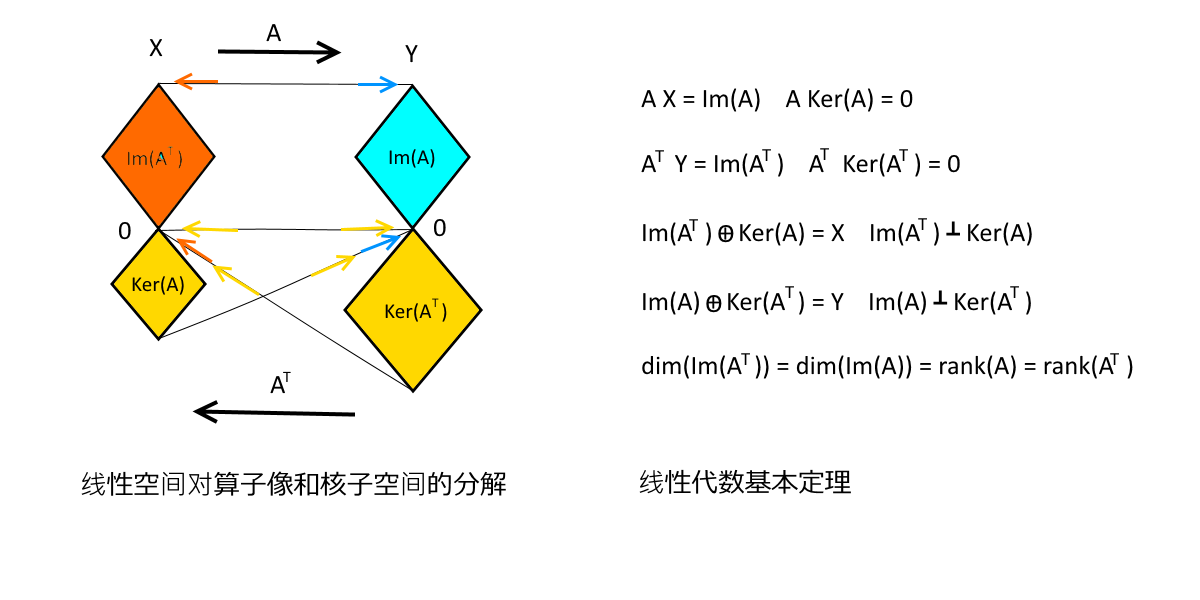
\includegraphics[width=0.7\linewidth]{pic/1604494yzy1do1yro41gva.png}
		\caption{线性代数基本定理}
		\label{1604494yzy1do1yro41gva}
	\end{figure}

	算子$ A $将核空间$ Ker(A) $中的向量映射为零向量,即矩阵中的行向量与它正交,而矩阵中的行向量张成转置矩阵的像空间$ Im(A^T) $。所以线性空间$ X $可以分解成正交的$ k $维子空间$ Im(A^T) $与$ n-k $维子空间$ Ker(A) $的直和,$ Y $可以分解成正交的$ k $维子空间$ Im(A) $与$ m-k $维子空间$ Ker(A^T) $的直和。这意味着$ X $的$ Im(A^T) $子空间中,线性无关向量在$ A $映射下的像也是线性无关的。对$ Y $也有相应的结论。
	\begin{gather*}
		Im(A^T)\oplus Ker(A)=X  Im(A)\oplus Ker(A^T)=Y
	\end{gather*}
	
	\subsection{线性空间和算子的不变量}
	
	线性空间的特征是\textbf{维数},它是空间中线性无关向量的最大个数,无论空间中的元素是什么具体的数学实体,同一维数的线性空间都对线性运算同构,都可以用相同维数坐标的列向量来表示。
	
	算子的\textbf{秩}是象空间的维数。$ n $维到$ m $维线性空间上的线性算子,在给定基的坐标下表示为一个$ m*n $矩阵。算子的象空间对应着矩阵列向量所张成的线性子空间,所以矩阵的秩等于它列向量中最大线性无关的个数。
	
	改变映射两边线性空间的基,表示线性算子的矩阵也随之改变。它们是同一个线性算子的不同表示,所以这些矩阵的秩都是一样的,秩是在基的变动中,矩阵表示保持不变的固有性质。
	
	空间中不同基之间对应着一个线性变换满映射,将一组基映射成另一组基,它可以表示为一个满秩的方阵。反之,满秩的方阵对应着两组基坐标间的变换。相同秩的$ m*n $矩阵,总是可以通过左右两边各乘以一个满秩的方阵变成一样。所以它们是同一个线性算子在不同基坐标下的矩阵表示。秩是$ m*n $矩阵在坐标变换中的不变量,它们对应着同一个线性算子。
	
	\subsection{无穷维线性空间}
	
	可以找到任意多个线性无关向量的线性空间,称为\textbf{无穷维线性空间},例如多项式空间,解析函数空间等等。我们知道所有解析函数都可以展开成泰勒级数,即等于无穷多个基向量的线性组合,是不是所有无穷维线性空间都能如此?
	
	大致是如此,但无穷多个基不一定都是可数的,也可能是连续谱的,其线性组合不限于无穷级数形式的和,还可能是积分形式的和。无穷多项的线性组合的含义,涉及到收敛和完备性的概念,这依赖于空间中的拓扑结构。
	
	代数只关心集合中元素运算的性质,而不涉及集合中元素的“相邻”和“远近”,这后者是拓扑关系,需在集合中另行定义。所以通常线性代数的课程只介绍有限维空间的向量和算子,这不需要了解空间拓扑的性质。但它的内容同样适用于无穷维的空间,只是涉及到向量“无穷和”时,需要收敛的概念。无穷维线性空间的内容多在泛函分析中介绍。
	
	我们脑中对向量想象的图像,通常是三维的几何空间,这是在实数域上以向量的内积赋予长度的概念,从而有可以度量远近的欧几里德空间。抽象的线性空间未必如此,所以我们以直观的图像想象抽象世界时,必须清醒地认识这些不同,头脑中“看到”的结果必须从定义出发用严谨的逻辑推理来验证它。
	
	在加法和数乘下封闭的一族函数集合是个线性空间,可以定义不同的“距离”,就有不同的收敛,例如点点收敛,一致收敛,几乎处处收敛等等。收敛性保证这无穷线性组合的分解有意义,完备性是说任何这类无穷线性组合的向量仍在这线性空间中。对此有兴趣可以看我“重修微积分”系列的博文。
	
	在无穷维线性空间中应用最多的是用内积定义距离完备的线性空间,称为\textbf{希尔伯特空间}。函数表示为傅立叶级数,贝塞尔函数级数等特殊函数都是在线性空间基上的分解。因为微分算子是线性的,在物理中许多微分方程都可以看成一个线性系统,而线性系统可以用叠加原理,当方程的解可以表示为一个函数族基向量的线性组合,微分算子作用在这些函数上仍然是它们的线性组合,微分方程以此化为代数方程组。这是在计算机时代前,历史上为微分方程的解法,发展出物理图像解释的数学根据。
	\chapter{重修线性代数6——行列式}
	行列式是线性代数中,联系线性方程组解,特征多项式和线性算子标准形式的一个枢纽。在西方科学史上,矩阵起先只是作为行列式所用的表示形式,线性代数的内容早就在这学科形成之前,在行列式的研究中已被了解了。行列式计算的解析表达式,是纯粹用代数方法来讲述这门学问的有力工具,但也因莫名其妙而饱受诟病。
	
	\section{行列式的几何含义}
	
	许多教科书都用莱布尼茨公式作为行列式的定义:
	\begin{gather*}
		\begin{vmatrix}a_{11}& a_{12}&\cdots& a_{1n} \\a_{21}& a_{22}&\cdots& a_{2n} \\ \vdots & \vdots&\cdots&\vdots \\a_{n1}& a_{n2} &\cdots& a_{nn}  \end{vmatrix} = \sum_{p}\sigma (p) a_{1p_1}a_{1 p_1}\dots a_{n p_n}
	\end{gather*}

	这里$ p=(p_1,p_2,\cdots, p_n) $ 是数组$  (1, 2,\cdots, n) $ 全排列中的一个置换,共有$ n! $个,$ \sigma(p) $是这置换的奇偶性,奇置换为-1,偶置换是1。这是个纯粹用算法程序来定义的函数,很难看出与经验关联足以想象的含义。这公式定义了行列式作为$ n $阶方阵中$ n^2 $个参数作为变量的多元函数,充满了对称的美、抽象方法的奇妙和构造性计算的确定性。也许教科书的作者想让学生,以此领略抽象代数中一些基本构件的联系,以及代数方法的简洁。但猛然来怎么一下,想看懂它和应用的联系,谁都觉得晕。
	
	在科学理论中列为范本的是欧几里德的几何原理,从简单的几条公理出发,纯粹用逻辑演绎出一套定理,无所不包地解释平面几何中一切关系。现代数学走向公理化的形式逻辑推理,抽象的代数方法无疑是最简洁和严谨的。却没去深思,几何研究面对的是图形,物理概念基于经验,抽象的美好来自于对已知具象的涵盖,驱动推理的灵感是心中的直观想象。除此之外,抽象的概念只是个符合定义条件的约束、什么都可代入的容器,逻辑推理只是句法的机械操作搬弄符号,无关语意,没有灵魂。所以符号主义的人工智能,缺乏人类联想的创作性和驱动推理的方向。高度抽象的数学,是到了高级阶段时对前面知识的总结,只在拥有了丰富的经验内容之后,才能显示出价值。对于初学线性代数的学生,用复杂的算法来定义一个重要的数学概念,会让人迷失在算法的程序中,与现实事物无从接轨。
	
	这里给行列式一个可以想象的几何含义的定义,让你能从图像中``看出''行列式的各种性质。
	
	行列式是用矩阵描写平行多面体广义体积的函数,以正负值来表示行列顺序在空间的定向。
	
	\kaishu
	
	在$ n $维空间中,$ n $个线性无关的向量$ x_1,x_2,\cdots,x_n $构成了一个平行多面体,它的广义体积是以这些向量为变量的多元线性函数$ V(x_1,x_2,\cdots,x_n) $,这函数有下列性质:
	
	1. 单位正交基向量的函数值等于1,$ V(e_1,e_2,\cdots,e_n)= 1 $. ($ n $维单位立方体的体积为1)
	
	2. 	如果变量中有两个向量相等,则函数值为0.(退化平行多面体的体积为0)
	
	3. 	体积函数对其变量具有线性关系,$ V(\cdots, ax+by, \cdots) = aV(\cdots, x, \cdots) + b V(\cdots, y, \cdots) $ 。
	
	\songti
	
	当$ n=2 $时,矩阵描写了平行四边形,$ n=3 $时,它是平行六面体,图形如下,你可以想象高维的情况。$ V $作为广义体积定义的性质,在线性空间的数域是实数时,符合经验的想象。
	
	\begin{figure}[h]
		\centering
		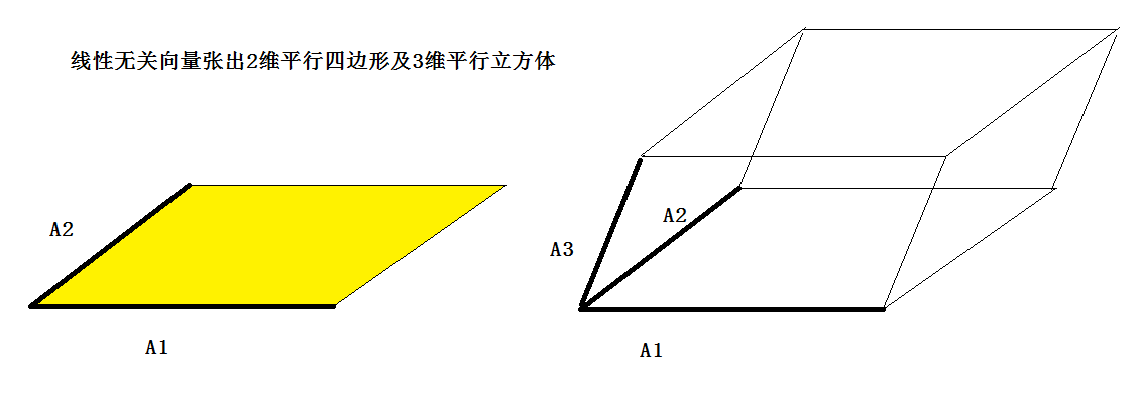
\includegraphics[width=0.7\linewidth]{pic/160908smn6gw0dy66yp37c.png}
		\caption{线性无关向量张出2维评选四边形及3维平行立方体}
		\label{fig:160908smn6gw0dy66yp37c}
	\end{figure}
	
	应用性质2和3,不难推导证明,若变量中两个向量对调位置,则$ V $函数乘上-1,这对应着在高一维的空间中,广义的体积作为与这平行多面体垂直向量的长度时它的朝向。
	
	向量$ x_1,x_2,\cdots,x_n $在标准正交基$ {e_1,e_2,\cdots,e_n} $上,表示为n个列向量$ A_1, A_2,$  $ \cdots,A_n $,用它们组成一个n阶方阵$ A = (A_1, A_2, \cdots,A_n) $,代入不难证明上面的莱布尼茨公式。
	
	列向量也可以直接看成是向量,把它们n个打包成方阵A,A的行列式表示为A到数域的函数,$ |A| = V(A_1, A_2,\cdots,A_n) $,函数值是这些列向量构成的平行多面体的广义体积。
	
	直接从行列式的几何定义出发,很容易想象,任何方阵如果其中的行向量或列向量是线性相关的,它们形成的平行多面体退化成一个低维空间上的几何体,体积为0。所以非零值行列式的矩阵的充要条件是满秩的。
	
	满秩的方阵可以分解为初等矩阵的乘积。任何方阵都可以分解成几个初等矩阵与对角线上只有1和0的对角阵。对角线上有0的对角阵对应着奇异的(不满秩的)方阵,即列向量线性相关,其行列式为零。单位矩阵行列式值为1。在这些初等变换中,数乘变换$ D_i(k) $把其中一个向量变长了k倍,面积也成k倍,列交换Pij改变了向量扫过平行四边形的方向,相反的方向乘上-1,而切变矩阵$ T_{ij}(k) $进行剪切变形,将j轴向i轴方向推斜了k:1斜度,保持体积不变,这些初等变换的行列式值分别等于k,-1,1,所以,方阵的行列式等于分解成的那些初等矩阵与对角阵行列式的乘积。因此,相乘的两个方阵行列式等于它们行列式的乘积。
	
	满秩方阵A的转置等于分解它初等矩阵和对角阵转置后的反向乘积 $ A^{'} $  $= (P_1 P_2\cdots P_k)^{'} = P'_k\cdots P'_2 P'_1 $,而对角阵的转置保持不变,初等矩阵转置后行列式不变,所以转置的矩阵行列式保持不变
	$ \left| A \right| = \left| {A'} \right| $。这意味着上面几何定义的行列式也可以用在行向量,所有对列操作运算的性质对行也适用。
	
	
	
	\section{代数余子式与向量的外积}
	
	中学数学里介绍过,三维向量a与b的外积是,它的结果是一个向量$ \textbf a \times \textbf b = \sin \theta \|\textbf a\|\|\textbf b \| \textbf n $,这向量的长度是由a和b形成的平行四边形的面积,方向n是与这平行四边形平面垂直,按右手定则确定的朝向。将这些向量表示成在i, j, k轴的分量形式,可以用行列式的式子来表示:
	
	\begin{gather*}
		\begin{pmatrix}a_1\\a_2\\a_3 \end{pmatrix} \times \begin{pmatrix}b_1\\b_2\\b_3 \end{pmatrix}= \begin{vmatrix}a_1&b_1&i \\a_2& b_2&j\\a_3&b_3&k \end{vmatrix} = \begin{vmatrix}a_1&b_1 \\a_2& b_2 \end{vmatrix}i - \begin{vmatrix}a_1&b_1 \\a_3&b_3 \end{vmatrix}j + \begin{vmatrix}a_2& b_2\\a_3&b_3 \end{vmatrix}k
	\end{gather*}

	这里的i,j,k分别是这些列向量作为坐标表示的单位正交基向量$ e_1,e_2,$  $e_3 $,这个外积向量在这些基向量的分量是这行列式的代数余子式,也可以看成把这两个向量分别投影到与这些基向量垂直的平面上平行四边形的面积。从三维空间中3个向量形成的行列式,可以推出
	
	\begin{gather*}
		\left (  \begin{pmatrix}a_1\\a_2\\a_3 \end{pmatrix} \times \begin{pmatrix}b_1\\b_2\\b_3 \end{pmatrix}\right )\cdot \begin{pmatrix}c_1\\c_2\\c_3 \end{pmatrix} = \begin{vmatrix}a_1&b_1&c_1 \\a_2& b_2&c_2\\a_3&b_3&c_3 \end{vmatrix}
	\end{gather*}

	这里$ \mathbf{a }\times \mathbf{ b} $表示平行四边形面积的法向向量,向量$ \mathbf{c} $对这法向向量的投影与平行四面体面积的乘积$ (\mathbf{a} \times\mathbf{b})\cdot\mathbf{c}$自然是这平行六面体的体积。这个几何的解释完全与行列式的计算一致。
	
	我们感兴趣的是怎么把这个几何直观推到n维空间。把这3个向量放在4维空间,依行列式的计算有
	\begin{gather*}
		\begin{vmatrix}a_1&b_1&c_1 &\textbf e_1\\a_2& b_2&c_2&\textbf e_2\\a_3&b_3&c_3 &\textbf e_3 \\0&0&0 &\textbf e_4\end{vmatrix}  = \begin{vmatrix}a_1&b_1&c_1 \\a_2& b_2&c_2\\a_3&b_3&c_3 \end{vmatrix} \textbf e_4
	\end{gather*}

	这说明行列式计算的广义体积,对应着在高一维空间中与这平行多面体垂直向量的长度。这向量可以用行列式表示为n个向量在n+1维空间上的广义外积。下面进一步解释细节。
	
	教科书都是用公式推导证明,n阶行列式可以按列(行)展开来计算,$ |A| = \sum_{i}a_{ij}D_{ij} $,这里的$ D_{ij} $叫做$ a_{ij} $的代数余子式,它是矩阵$ A $中划去第$ i $行第$ j $列后n-1阶行列式的值乘上$ (-1)^{i+j} $。这低一阶的行列式如法炮制,又可以用再低一阶的行列式来计算,这种递归算法叫做拉普拉斯定理。然而,从几何解释中直接看出这一点,将给我们更清晰的图像理解。
	
	对应着A的第j列向量$ A_j $的代数余子式$  (D_{1j},D_{2j}, \cdots, D_{nj})^T $组成代数余子式向量$ D_j $,行列式$ |A|=A_j\cdot D_j $。从行列式是广义体积的几何图像来看,$ D_j $就是n维$ A $矩阵中,除去$ A_j $余下的n-1个向量,张成n-1维空间里平行多面体的广义体积。这n-1维的广义体积的向量与它所在的子空间垂直,它与$ A_j $的内积作为``面积''与``高''的相乘,构成n阶行列式的广义体积。
	
	代数余子式向量可以看做三维空间中两个向量外积概念的推广,从三维空间中两个向量平行四边形面积为长度的法向向量,推广到n维空间n-1个向量平行多面体广义体积为长度的法向向量。代数余子式$ A_{ij} $是对应于j的法向向量对第i坐标轴的投影,这法向量与多面体所在的子空间垂直,相当于这多面体向与第i坐标轴垂直的子空间的投影,所以在计算广义体积时,不计这n-1个向量在第i坐标轴上的分量,在构造余子式的n-1阶子行列式中,需要移动矩阵A的第j列移和第i行到子行列式外,其中交换列和行$ 2n-i-j $次,所以代数余子式要乘上$ (-1)^{i+j} $因子。
	
	一般形式的拉普拉斯定理,把这种三维空间中``高''与``面积''的相乘得到``体积''的思路,进一步推广到n维空间广义体计算积中,用k阶行列式的子式表示的投影到``高''那k维部分的向量,与n-k阶代数余子式表示的``面积''部分向量的内积。
	
	如果你还没有形成足够的空间想象能力,能通过上面的描述看到几何图像,建议用上面二维和三维空间行列式和向量外积计算,在纸面上画出图形来理解。线性代数课是继平面几何,解析几何之后,对抽象的空间想象能力的训练。抽象概念的想象也是在课程学习中,逐步建立起来能够看到的画面,在学习中忽视了这一点,你就无法看到进一步学习内容中的图像。
	
	\section{逆矩阵和克莱姆公式}
	
	矩阵$ A = (\mathbf{A_1},\mathbf{ A_2}, \cdots,\mathbf{A_n}) $的代数余子式向量构成的矩阵$ D = (\mathbf{D_1}, \mathbf{D_2},$  $\cdots,\mathbf{D_n}) $的转置,叫做$ A $的伴随矩阵。代数余子式向量与张成它的n-1阶多面体垂直,$ D_i·A_j = 0,i \neq j $;由拉普拉斯定理有$ D_j\cdot A_j = |A| $,所以$ D^TA = |A|I $,这得出非奇异方阵的逆的解析表达式$  A^{-1} = D^T/|A| $。
	
	对于线性方程组$  Ax = c $,将$ A $的伴随矩阵左乘方程两边,则得到$ |A|x = (D_1, D_2, \cdots,D_n)^Tc $,所以x的第i个分量有$ |A|x_i = D_i\cdot c $,由6.2节中拉普拉斯定理的解释得知这个内积等于行列式$ |D_1, D_2,\cdots D_{i-1},c,D_{i+1},D_n| $,当$ A $是非奇异时则有克莱姆公式$ x_i=|D_1, D_2, \cdots D_{i-1},c,D_{i+1},D_n|/|A| $。
	
	行列式是个有确定结果的算法表达式。无论是求矩阵的逆还是线性方程的解,以及以后的各种应用,都能用它得出解析的式子,这在理论上有很大意义。但是由于它的计算量与其阶数成指数函数关系,所以除了2阶等极端情况外,在实践中都是先将矩阵变换成三角阵或准三角阵后再行计算。
	
	\section{张量和半张量积}
	
	行列式的值对于它的列向量(或行向量)都有线性关系,它可以看成是一种斜对称的多线性函数,向量的内积是两个变量的对称双线性函数。研究多线性代数的数学称为张量分析。张量是用来表示在标量、向量和其他张量之间线性关系的多线性函数。它是一种比向量更广泛意义上的``数量'',它的概念可以包括标量、向量、线性算子等等作为特殊情况。在线性空间上线性作用的重数称为张量的``阶(rank)'',标量可以看作是0阶的张量,向量是1阶的,线性算子是2阶的。在给定的坐标下,向量表示为1维的数组(即列向量),线性算子为2维的数组(即矩阵),r阶张量为r维数组。在坐标变换中依变换的方式不同,其指标可以分成协变和逆变两种,具有丰富的表达能力,在物理和工程上有着广泛的应用。
	
	高维数组在数学和工程问题上经常使用,尤其应用在对多线性和非线性问题的处理,但在显示和分析上十分不便。如果把它们按一定的顺序排成一列或矩阵,规定它们间合适的运算规则,则既可以方便地在书面上显示、作理论分析,又能与原来的数组运算等价。这种新的矩阵运算叫做``半张量积'',是对普通矩阵乘法进行推广。传统上矩阵的乘法AB,要求A的列数与B的行数相等,相乘时A 与B中的相应的元素是1对1的运算;矩阵的张量积没有这限制,它是A中的每个元素与整个B矩阵来相乘,但它与传统矩阵乘法不能兼容;而半张量积与张量积一样,对A、B矩阵的列行数并无要求,其运算规则介乎传统乘法与张量积之间,当列行数相等时即为传统的矩阵乘法,但有倍数关系时就变成其中一个矩阵元素与另一矩阵按倍因子分块配对的乘法,进而推广到任意的两个矩阵。半张量积的这种矩阵运算规则,不仅适用于多维数组排成矩阵后的等价运算,而且它与矩阵的加法有分配律,与矩阵通常乘法有结合律,这是一种漂亮地解决多维数组书面表达、分析、计算和扩展矩阵乘法的设计。这是程代展教授对矩阵理论的原创性贡献,经过十多年普及,现已成为表达有限集合上映射及性质,研究有限集合上的动态系统的演化规律及控制的有力工具,在动力系统、网络、线路设计与检测等方面有许多应用。\\
%\\[12pt]
	
	【补充】贴在评论[10]之后
	
	一些读者对半张量积好奇,希望给个简单的例子。这里简介一下。
	
	定义:设A是$ m\times n $矩阵,B是$ p\times q $矩阵,记$ n $与$ p $的最小公倍数为$ t  $. 定义$ A $与$ B $的半张量积为
	\begin{gather*}
		  (A\bigotimes It/n)(B\bigotimes It/p) 
	\end{gather*}
	这里$ \bigotimes $是矩阵的张量积(Kroneckerproduct)。
	
	注:上述定义中,如果n=p称A与B是等维数,如果n与p其中一个能整除另一个,则称是倍维数的, 其他为一般情况。定义是对一般情况给出的。对于等维数的情况, 它退化为普通矩阵乘法,倍维数可简化为分块积。因此, 半张量积是普通乘法的推广。倍维数情况定义左半张量积是最常用的。在这定义下结合律与分配律对半张量积仍成立。
	
	仍然觉得晕?好吧,举例说明。张量积$ A\bigotimes B $意思是A中每一个元素与每一个B中元素相乘的矩阵,或者说A中每一个元素与整个B相乘,然后按A的布置排出的矩阵,比如说:
	\begin{gather*}
		B=\begin{pmatrix}1 &2 \\-1&3\end{pmatrix},I_2=\begin{pmatrix}1 &0\\0&1\end{pmatrix},B\bigotimes I_2=\begin{pmatrix}1 & 0 &  2& 0\\ 0 & 1 &  0& 2\\  -1&  0&  3& 0\\ 0 & -1 &  0& 3\end{pmatrix}
	\end{gather*}

	假如A是3x4的矩阵,B如上是2x2的矩阵,它们的最小公倍数是4,I1是1,A与B的半张量积 $ A\circledast B $ 如下(注:$ \circledast $ 不是半张量积的标准符号,只是无法找到这标准符号,暂时用它聊以示意)
	\begin{gather*}
		A=\begin{pmatrix}1 & 2 & -1& 2\\ 0 & 1 &  2& 3\\  3&  3&  1& 1\end{pmatrix}, A\circledast  B = A(B\bigotimes I_2)=\begin{pmatrix}2 & 0 & -1& 10\\ -2 & -2 & 6& 11\\2& 2& 9& 9\end{pmatrix}
	\end{gather*}
	
	因为这是倍维数的半张量积,也可以把它化简为A中的列分成2块与B向乘。
	\begin{gather*}
		A_1=\begin{pmatrix}1 & 2 \\ 0 & 1 \\  3&  3\end{pmatrix}, A_2=\begin{pmatrix} -1& 2\\ 2& 3\\ 1& 1\end{pmatrix},\\
		A\circledast B =\begin{pmatrix}A_1 & A_2\end{pmatrix}\begin{pmatrix}1 &2 \\-1&3\end{pmatrix}=\begin{pmatrix}A_1-A_2 & 2A_1+3A_2\end{pmatrix}=\begin{pmatrix}2 & 0 & -1& 10\\ -2 & -2 & 6& 11\\2& 2& 9& 9\end{pmatrix}		
	\end{gather*}

	为什么定义这样的乘法?想一想A原来是个3x2x2的三维数组展成的矩阵,A1,A2是三维数组的第三个下标的两个断面,为了显示方便把它们并排放一起变成一个矩阵,这第三个下标方向按传统方式与B来相乘(想象一下线性算子的复合),然后再把它们排放成一个矩阵。想进一步了解它的理论和应用,详见:
	
	1. 程代展, 赵寅. 矩阵的半张量积: 一个便捷的新工具. 科学通报, 2011, 56: 2664–2674
	
	2. 程代展,齐洪胜,矩阵的半张量积理论与应用,科学出版社,2007
	\chapter{重修线性代数7——相似}
	把向量看作是状态,线性变换驱动着线性空间中所有向量的变化,从一个状态变为另一个状态,如在空间中运动。对于一个具体的线性算子,从对空间不同方向的影响来剖析算子的特性,便可以从抽象的高度俯视算子在不同坐标表示矩阵的共同性质,从中选择合适的视角便能看到算子的结构。
	
	线性变换的矩阵表示是一个方阵。这线性变换在旧的基下的矩阵表示$ A $,在新的基下表示为$ T_{-1}AT $. 对于线性变换,秩仍然是在不同基的坐标表示中不变量,但把映射限制在原来的空间。仅仅是相同秩的方阵,不足以通过坐标变换而相等。同一个线性变换在不同坐标下表示为不同的矩阵,称为是\textbf{相似}的,相同秩的方阵并非都是相似的。这里介绍怎么通过线性变换的不变子空间,理解相似矩阵标准形式的直观意义。
	
	\subsection{不变子空间}
	
	对于线性空间正交基,每个基向量张成一个一维子空间,线性空间是这些一维子空间的直和。向量的坐标值分别对应着它在每个一维子空间的分量。线性空间只要选取合适的基,就可以做出所需的子空间直和的分解。对于线性空间中的线性变换,并非任意的子空间能对线性变换保持封闭,最有意义的是对线性变换是封闭的子空间分解。
	
	如果一个线性子空间对一个线性变换保持封闭,即子空间中任何向量经过这变换仍在这子空间中,则它称为这个线性变换的\textbf{不变子空间}。线性变换对它不变子空间上向量的作用,等于它局限在这个较低维数线性算子的作用。所有线性变换所得的向量形成一个子空间,称为线性变换的像。所有在线性变换下映成零向量的向量集合也是一个子空间,称为线性变换的核。线性变换的像和核都是它的不变子空间。
	
	设K是线性变换$ \alpha $ 的一个不变子空间,线性空间N的维数是n,K的维数是k,取K的基为N的基中前k个基向量,线性变换$ \alpha $在这基上的矩阵A,它的前k个列向量对应着K中的基向量在线性变换下的线性表示,而K是$ \alpha $的不变子空间,这意味着,这k个列向量,除了前k个分量外,其余的都为0. 方矩A具有下面的形式。
	\begin{gather*}
		A = \begin{pmatrix} B & C\\0 & D\end{pmatrix}
	\end{gather*}
	这里B是k阶方阵,它是线性变换$ \alpha $在K子空间(这个基)上的矩阵表示。
	
	如果与K正交的子空间J也是$ \alpha $的不变子空间,那么在它们的基下,矩阵A可以表示为对角方块形式
	\begin{gather*}
	A = \begin{pmatrix} B & 0\\0 & D\end{pmatrix}
	\end{gather*}
	这样计算和分析都更为简单。可惜这并不总是能够做到的。消化了这方面内容的读者,自己应该能够举出例子。
	
	\subsection{若当(Jordan)标准形式}
	
	线性变换在给定的基上表示为一个矩阵,n维线性空间上的线性变换为n阶方阵。相似的矩阵A和B,是同一个线性变换在不同基上的表示,两个基坐标之间的变换是$ T $时,$ B= T_{-1}AT $。我们研究怎么选取一个合适的基将线性变换表示为一种简单的矩阵形式,也就是对于给定的方阵,怎么通过合适的坐标变换变成统一且方便的形式。
	
	显然,矩阵中含有越少的非零元素就越容易计算和分析,对角阵或具有较小方块的准对角阵是个很好的选择。从上面看到,用不变子空间的向量作为基,线性变换在这基上的矩阵可以表示为上三角形分块矩阵,如果空间可以分解为不变子空间的直和,则矩阵可以相应表示为准对角线矩阵。我们看看如何将已有的矩阵变成尽可能小方块的准对角阵。
	
	先从特征向量入手。
	
	线性变换$ \alpha $ ,如果它有一维的不变子空间。则这子空间里的向量r,称为是线性算子$ \alpha $的特征向量,这时有$  \alpha r  = \lambda r  $,这个线性空间的数域中标量$ \lambda $,称为是$ \alpha $ 的特征值。对于线性变换 $ \alpha $ ,如果n维线性空间有n个一维的不变子空间,用这些不变子空间的向量为基,$ \alpha $ 就可以表示为一个对角阵,对角线上元素是相应的特征值。这是最美好的情况。这样的矩阵称为可对角化。能够被酉变换下对角化具有特别意义。
	
	正规性是检验矩阵能否在酉变换下对角化的简单方法,矩阵$ A $如果与自己的共轭转置$ A^{*} $的乘法是可交换的,即$ A^*A  = AA^* $,则称为它是正规矩阵。正规矩阵可以经酉变换对角化,反之,能通过酉变换与对角阵相似的必然是正规矩阵。矩阵是正规的当且仅当其特征向量能张成整个空间,且相互正交。厄米矩阵是正规矩阵,所以它能够对角化,而且特征值都是实数,特征向量相互正交。
	
	可惜这并非都有可能,线性变换可能有多个一维不变子空间,即多个特征向量和特征值,也可能只有一个。但这是一个很好的思路。
	
	给定一个线性变换的矩阵表示A,怎么求它的特征值和特征向量?这是解线性方程组$ Ax=\lambda x $的问题,这里向量x和标量$ \lambda $都是未知的。把这方程改写成 $ (A – \lambda I)x = 0 $的形式,这里I是单位矩阵,如果行列式 $ |A – \lambda I| = 0 $,这个齐次方程组有解。我们知道,n阶矩阵行列式$  |A – \lambda I| = 0 $是个$ \lambda $为未知数n次代数方程,叫做特征方程,对于复数域,这多项式的特征方程有n个根,这些根都是矩阵A的特征值,而对应$ \lambda $值的齐次方程解则是特征向量。

	如果矩阵A有n个不同的特征值,这些特征值为对角线的对角矩阵D是A的相似矩阵,不难证明相应的特征列向量是线性无关的,它们排成坐标转换的矩阵T,我们有$ T^{-1}AT = D $.

	但是这n个特征值并非都是不同的,对于k重根的特征值,对应的齐次线性方程不一定有k个线性无关的解,即所有的特征向量不足以张成全空间。所以在有重根的情况,A也许不能与对角阵相似。在这种情况下,它总可以表示为准对角阵。大致说来,代入k重根特征值的矩阵$ (A –\lambda I)^k $表示的是一个线性变换,它的核是A的一个k维不变子空间。我们可以选取这子空间合适的基,将A代表的线性变换表示为对角线上元素是$ \lambda_i $的一些若当块$ J_i $矩阵。线性空间可以分解为不同特征值$ \lambda_i $所对应的不变子空间的直和,所以A可以通过坐标变换表示为对角线上元素为特征方程解$ \lambda_i $的若当标准形式矩阵J.
	\begin{gather*}
		J={\begin{bmatrix}J_{1}&\;&\;\\\;&\ddots &\;\\\;&\;&J_{p}\end{bmatrix}},  \;\;\; J_{i} = {\begin{bmatrix}\lambda _{i} &1&\;&\;\\\;&\lambda _{i}&\ddots &\;\\\;&\;&\ddots &1\\\;&\;&\;&\lambda _{i}\end{bmatrix}}, \;\;i=1,2,\cdots,p
	\end{gather*}

	\subsection{有理标准形式}
	
	如果线性空间的数域不是复数,n阶特征方程不一定都能得到n个根,这种情况下线性变换不能表示为若当标准形式。我们寻找另一种方法,也能把线性变换表示成非零元素非常少的矩阵。
	
	对于n阶矩阵A所表示的线性变换,假设可以找到一个向量r,线性变换A逐次施加其上,得到n个不相关的向量,即循环向量集$ {r , Ar, A^2r, \cdots, A^{n-1}r} $,构成了线性空间的基,那么$ A_{n}^{r} $一定与它们线性相关,$ A^{n}_{r} +a_{n-1} A^{n-1}_r + \cdots + a_1A_r+ a_0r = 0 $,这个线性变换在这基上可以表示为矩阵R:
	\begin{gather*}
		\begin{pmatrix}0 &0& \cdots &0& -a_{0}\\ 1 &0& \cdots &0& -a_{1}\\ 0 &1&  &0& -a_{2}\\  \vdots & \vdots &\ddots & \vdots\\ 0 &0& \cdots & 1& -a_{k-1} \end{pmatrix}
	\end{gather*}

	这个矩阵R称为多项式$  p(x) =x_n +a_{n-1}x_{n-1} + … + a_1x + a_0 $的伴侣矩阵,它是一个有理标准形式,可以在线性空间所在的任何数域上实现。循环列向量集 $ {r , Ar, A^2r, …, A^{n-1}r}  $是新的基在旧的基上的表示,它排列构成的矩阵T是新旧坐标的变换,我们有 $ R = T^{-1}AT $,即R是A的相似矩阵。
	
	现在的问题是:是否存在着这样的向量r?如果存在,不同的r生成的基上,与矩阵A相似的有理标准形式是否一样?
	
	记$ m(x) = x^k+a_{k-1}x^{k-1} + … + a_1x + a_0 $,称m(x)为A的最小多项式,如果m(A)=0是能够让多项式矩阵变成零的最小阶次。第一个问题答案是:如果n阶矩阵A的最小多项式是n次,那么存在着一个向量,A对它的循环向量集形成线性空间的基。
	
	这个并不难证明:A的n次矩阵多项式为零,意味着任何向量在A的n次重复作用下线性相关,而最小多项式说,不可能让所有的向量在比它少次数的重复作用下线性相关,所以在这种情况下总有一个向量r,它A对它的循环向量集构成空间的基。
	
	伴侣矩阵是由A的最小多项式确定的,它与生成基的向量无关。所以由不同的r用A重覆作用生成的基上,矩阵的有理标准形式都是一样的。
	
	怎么能得到最小多项式呢?对于n阶矩阵A,行列式 $ p(x)  = |A – xI| $是$ x $的 $ n $次多项式,Cayley-Hamilton 定理告诉我们,这特征多项式矩阵p(A) = 0,所以A的最小多项式必须是它的因子。另一方面,特征多项式的根是A的特征值$ \lambda $,它也必须是最小多项式m($ \lambda $)的根。这是因为,特征值所对应的特征向量y,在A的最小多项式作用下$  m(A)y = m(\lambda)y $ ,除非$ m(\lambda)=0 $,不然它不等于零向量,这与最小多项式的定义矛盾。这两个性质告诉我们,如果特征多项式没有重根,它就是最小多项式,否则我们可以用A代入计算,确认它是否最小多项式。
	
	如果特征多项式不是最小多项式,我们不能将线性变换表示为一个特征多项式的伴侣矩阵的形式。但可以把它表示为有理标准形式的矩阵,即对角线上是几个多项式伴侣矩阵的准对角阵。大致说来,这时最小多项式m(A)的次数是k,$ k  \textless n $,意味着有一个向量,A对它的循环向量集有k个,以此为基构成了A的k维不变子空间。在这不变子空间里,算子在这基上表示为它的伴侣矩阵。假设线性空间被线性变换A为分解成几个不变子空间直和,$ m1(A), m2(A),$   $\cdots, m(A) $分别是A局限在这些子空间上的最小多项式,局限在这子空间里线性变换A的最小多项式必须是全空间最小多项式的因子,所以有 $ m1(x) | m2(x) |$   $\cdots | m(x) $ . 特征多项式在不同的基上保持不变,则有$ p(x)= m1(x) m2(x) \cdots$   $m(x) $,在简单情况下可以得出这个有理标准形式。
	
	\subsection{$\lambda$矩阵}
	
	上面两小节告诉我们,如果矩阵A的特征多项式没有重根,对于复数域,A可以与对矩阵相似,对于任何数域都可以与特征多项式的伴侣矩阵相似,它们分别对应着A所代表线性变换的若当标准形式和有理标准形式。A与相似的标准形式间的坐标变换矩阵,可以直接由相应的特征向量,以及循环向量集组成。
		
	对于多项式有重根的情况,虽然我们大致了解怎么形成这两种准对角阵的标准形式,但是严格的证明必须引入$ \lambda $ 矩阵,初等因子,不变因子等概念才能说清。
		
	到了要说清线性变换矩阵的标准形式,线性代数或矩阵论到了学习抽象方法的一个关口。课文在这之前,多数已经介绍群、环、域、多项式和行列式等等概念和性质,在这里把它们综合起来解决这个问题。很多人在这之前多已迷糊了,为什么东一榔头,西一锤子零散着介绍许多概念,又不深入介绍它们的应用,布了这么一大的局,最后绕圈子的证明实在让人晕乎。能有更简单直接的证明吗?应该会有,但课文的目的是趁机介绍这些抽象代数基步的概念,并用这个标准形式的证明作为抽象方法的例子。这部分内容的理解大约是课文中最艰深理论的部分,过去对于物理和微分方程的理论分析十分重要,但现在对绝大部分工科学生却不是最有用。我只在这里大致介绍一下它们间的联系。
	
	前面介绍的矩阵的元素都是在数域上,称为数字矩阵。如果矩阵上的元素是个$ \lambda  $的多项式,即线性空间定义在数域的多项式环上,例如用行列式求矩阵特征方程的特征矩阵 $ A -\lambda I $,这样的矩阵称为$ \lambda $ 矩阵。对矩阵对换行(列),数乘一行(列)以及数((相应地用多项式)乘一行(列)加在另一行(列)中称为矩阵的初等变换,通过初等变换把一个矩阵变为另一个矩阵,称这两个矩阵是等价的。定理证明,$ \lambda $ 矩阵都可以通过初等变换,变成只有对角线上是非零的矩阵,对角线上的元素($ \lambda $ 多项式)从上到下依次有$ d1(\lambda ),d2(\lambda ),\cdots,ds(\lambda ) $,余下是0,这些非零多项式称为$ \lambda $ 矩阵的不变因子,前面不变因子能够整除是后面的不变因子,即$ d1(\lambda )|d2(\lambda )|\cdots|ds(\lambda ) $,能够同过初等变换成这样形式的矩阵是唯一的,称为等价矩阵的标准形式。所以具有相同的不变因子是矩阵等价的充要条件。
	
	定理证明,矩阵A和B相似的充要条件是特征矩阵(A-$\lambda$ I)与(B -$\lambda$ I)是等价的,即它们的特征矩阵的不变因子都是相同的。
	
	每个不变因子是个$\lambda$ 的多项式,它对应着一个伴侣矩阵,即多项式的伴侣矩阵的特征矩阵是个对角线上最后一个元素是这个多项式,其他都是1的对角阵。所以与矩阵相似的有理标准形式是个准对角阵,对角线上依次对应着其特征矩阵每个不变因子的伴侣矩阵。
	
	对于复数域,每个特征矩阵上不变因子可以分解为互不相同特征值的幂次因子,例如$ d_k(\lambda ) = (\lambda - a_1)^{k1} (\lambda - a_2)^{k2},(\lambda - a_m)^{km} $这样相乘的每个幂次因子称为初等因子,所以复数域上矩阵相似的充要条件是特征矩阵的初等因子是相同的。
	
	不难验证每个初等因子唯一对应着一个若当块,所以复数域上矩阵都能与若当标准形式的矩阵相似。当特征矩阵的初等因子都是一次时,矩阵能够与对角阵相似。
	\chapter{重修线性代数8——分解 }
矩阵的分解,实际上是通过坐标变换来揭示矩阵所表示的线性算子性质。

在过去,人们靠公式的推导来简化计算,线性代数主要用在理论分析和解方程,其重点是表达线性变换的特征,在不同坐标上矩阵表示的相似性和标准形式。在计算机时代,人们关心矩阵的线性运算特征,抽取矩阵的线性放大特性和近似,应用于海量的数据存储和计算。代表着线性算子的一般矩阵的分解,特别是SVD分解,便成为今日关注的重点。

\section{满秩方阵的分解}
满秩的方阵对应着一个坐标变换,它可以分解为几个初等变换的乘积。这个分解的目的,在于计算上通过这些初等变换的操作,来解方程和求逆。

我们知道,对线性方程组,调换组中方程的次序,在方程的两边同乘以非零的数,以及将一个方程乘数,两边同加在另一个方程上,都不改变方程组的解。

从线性空间角度来看,这不过是在值域空间做坐标变换。方程的解x是b在矩阵列向量的线性组合系数,改变了这些向量的坐标表示,当然不改变b与矩阵列向量的线性表示关系。

我们把上面三种对方程组的操作称为初等变换,即:(1)两行(列)互换:$ \mathbf{R}_{i} \leftrightarrow \mathbf{R}_{j} $,(2)把某行(列)乘以一非零常数:$ k\mathbf{R}_{i}\rightarrow \mathbf{R}_{i} $ , 其中$ k\neq0 $,(3)把第i行(列)加上第j行(列)的k倍:$ \mathbf{R}_{i} + k\mathbf{R}_{j}\rightarrow \mathbf{R}_{i} $。初等矩阵即是将上述3种初等变换作用到单位矩阵的结果,分别记为  $ P_{ij},D_{i}(k),T_{ij}(k) $,对应于旋翻、缩放($ k=-1 $为翻转)和剪切的变换。初等变换对应于一个坐标变换,初等矩阵左乘矩阵A,则是对A行的变换,它相应于算子A的值域空间中的坐标变换。初等矩阵右乘矩阵A,则是对A进行列的变换,它相应于在算子A的定义域空间中坐标变换。

读者不难在头脑中想象到初等变换的矩阵形式,初等矩阵都是满秩的线性变换。从变换的含义马上得出它们的逆矩阵分别是$ P_{ij},D_{i}(1/k),T_{ij}(-k) $。

参考一下解方程中的高斯消去法,对于一个方阵A,它可以一系列行的初等变换,把它变成上三角阵$ U $,即$ P_{1}P_{2}\cdots P_{s}A=U $,因为这些是初等矩阵,很容易写出逆来相乘$ P_{s}^{-1}\cdots P_{2}^{-1}P_{1}^{-1}=L $,显然$ A = LU $. 消去法没有换行时,P都是下三角阵,则L是一个对角线都是1的下三角阵,这便是\textbf{LU分解}。三角阵的线性方程可以用迭代法求解,这个分解用来解方程和求行列式。

不难想象k秩的矩阵A,可以等价于对角线上左上角开始有k个1,其余都是0的矩阵。如果A是一个满秩的矩阵,它等价于单位矩阵。

对于n阶满秩方阵A求逆的计算,因为A的逆是一系列把它变成单位矩阵I的初等矩阵的乘积,把n阶单位矩阵拼在A的右边成为$ n\times 2 n$的增广矩阵$ (A\ I)$,然后对它进行初等行变换,直至左边的$ n\times n $那块是单位矩阵,右边那$ n\times n $部分就是A的逆。这个计算过程相当于$ A^{-1}(A\ I)=(I\ A-1) $。

\section{正交变换}

一般线性空间中坐标变换,在欧几里德空间里,包含着坐标的拉伸、旋转、翻转、剪切等变换,坐标轴之间可能是倾斜。这对只关心加法和数乘代数性质的线性空间,并没有什么关系。因为这抽象线性空间,根本没有``拉伸''和``倾斜''等几何的概念。长度和角度概念由内积运算定义的,要讲究这些,必须在内积空间里来谈论。

保持内积不变的坐标变换,也就是向量的长度和夹角,在不同坐标系上的表示都保持不变。这种坐标变换称为正交变换,物理上称么正变换。它的矩阵在实数域是正交阵,在复数域是酉阵。这直接可以从对偶算子和内积等式推出$ \langle y, \bar{x}\rangle=\langle Uy, Ux\rangle=\langle y,U^{*} Ux\rangle \rightarrow U^{*}U=I $,在实数域$ U^{*} = U^{T}  $. 以后我们都只在实数域上讨论,对于复数域,将转置换成共轭转置就行。

内积空间坐标表示必须在标准正交基上,这样才能保证同构关系。正交变换是把这各向同性直角坐标系,刚性地整体旋转和翻转,所以表示的向量长度和夹角在变换后保持不变。

对于线性变换的方阵,坐标变换是同样作用在算子的输入和输出空间,因为在内积空间上坐标变换必须是正交变换,在线性空间上相似的矩阵,在内积空间上未必做得到。例如非对称的矩阵有可能与一个对角阵相似,但未必有正交的坐标变换做到这一点。在内积空间(通过正交变换)与对角阵相似,当且仅当它是正规矩阵,正规矩阵A有$ A^{*}A  = AA^{*} $. 实数域上的对称阵和复数域上的厄米矩阵都是正规矩阵。

对于$ m\times n $矩阵A, $ m\ge n $可以分解成列向量的$ m\times n $单位正交集Q与一个$ n\times n $的上三角阵R相乘, $ A=QR $,这叫做\textbf{QR分解}。这个分解可以看作依次按照Gram-Schmidt方法对A中的列向量做正交化,Q就是单位正交化后的列向量,R中的元素是正交化过程中的内积。矩阵Q表现旋转和翻转部分的映射,R体现了缩放和剪切的畸变。

怎么把线性无关的列向量变成单位正交的向量组?这在几何上很直观。取矩阵A的第一个列向量$ A_1 $把它标准化(归一化) $ e_1 = A_1/\|A_1\| $ ,其中的长度放在R阵的第一个对角线元素上 $ R_{11}=\|A_1\| $,再取第二个列向量$  A_2  $,减去它在$ e_1 $的投影的向量$ x_2 = A_2 - \langle A_2, e_1 \rangle e_1 $,令 $ R_{12}=\langle A_2, e_1 \rangle $,再把它标准化$ e_2 = x_2/\|x_2\| ,\;\;R_{22}=\|x_2\|,\;\;e_1, e_2 $ 便是两个标准正交的向量。已经有了k-1个标准正交向量,取第k个列向量$ A_k $,减去它在这些标准正交向量的投影向量 $ x_{k} = A_{k} - \sum_{i=1}^{k-1} \langle A_{k}, e_i \rangle e_i $ ,将这些投影分别放在R阵中 $ R_{ki}= \langle A_k, e_i \rangle $ ,再把它标准化$ e_k = x_k/\|x_k\|, \; R_{kk}= \|x_k\| $,如此下去。这个过程叫做Gram-Schmidt正交化。显然,标准正交的向量构成Q矩阵 $ (e_1, e_2,\cdots ,e_n)=Q $,R是一个上三角阵,A=QR。对于矩阵的列向量不是线性无关时,Q阵略去0向量,最后添上与前面正交的标准向量。

在MATLAB和Octave中,用qr函数来计算行QR分解,指令为:[Q,R]=qr(A),分解为m*m的Q阵和m*n的R阵。

\section{线性算子对核与像空间的分解}

前面介绍过,表示线性算子的矩阵A,它的核Ker(A)是所有映射成零的向量集合,构成了X中的一个子空间;它的像Im(A)是所有映射得到向量的集合,构成了Y中的一个子空间。我们有线性代数的基本定理,表示为下图。

% TODO: \usepackage{graphicx} required
\begin{figure}[h]
	\centering
	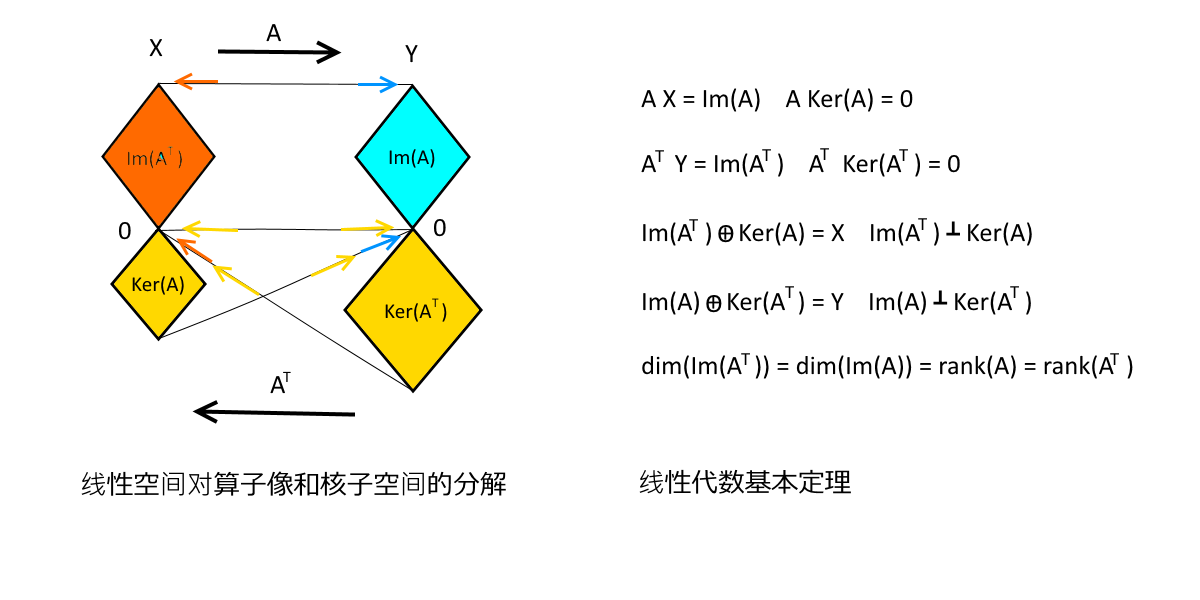
\includegraphics[width=0.7\linewidth]{pic/1604494yzy1do1yro41gva.png}
	\caption[代数学基本定理]{线性空间对算子像和核空间的分解}
	\label{fig:1604494yzy1do1yro41gva}
\end{figure}


算子A将输入空间X和输出空间Y,分别分解为正交的两个子空间的直和。

\[ Im(A^T)\oplus Ker(A)=X   Im(A)\oplus Ker(A^T)=Y"  \]%width="501" height="20" style="width: 501px; height: 20px;

X的线性子空间$ Im(A^T) $和Y的$ Im(A) $有相同的维数k,说明$ Im(A^T) $的基向量在算子映射下的像可以作为$ Im(A) $的基向量,算子A局限这子空间中,在这两个基的矩阵表示是k阶单位向量。

在$ Im(A^T) $子空间选取k个线性无关的向量 $ {V_1,V_2, \cdots,V_k} $,在Ker(A) 选取n-k个 $ {V_{k+1}, \cdots,V_n} $,共同构成X的一个基。令$ U_i= AV_i, i=1, 2, \cdots,k $,它们构成子空间Im(A)的基,在Ker(AT) 选取m-k个$  {U_{k+1}, \cdots,U_n} $,共同构成Y的一个基。在这两个空间的基上,线性算子$ \alpha $表示表示为主对角线上前r个是1,其他全是0的``k秩准单位阵''D。

\[U^{-1}AV = \begin{pmatrix}I_k&0\\0&0\end{pmatrix}\]

秩数为k的线性算子在合适的基上都可以表示为``k秩准单位阵'',即k秩的矩阵A可以分解成 $ A = UDV^{-1} $,D是与A的行列数秩数相同的``准单位阵'',V和U分别是X和Y空间里新旧坐标的变换矩阵。注意到构造V和U时基时,除了要求前k个$ U_i = AV_i $,外,其他的基向量是在指定的子空间内,任意选取线性无关的即可,所以除了D是由矩阵的秩唯一确定之外,有无数个不同U和V的分解。

\section{奇异值分解}

线性算子对核和像空间的分解只是简单地区分对算子的映射值``有影响''和``无影响''的两部分。许多的应用希望了解线性算子作用在不同方向的放大特性,这涉及到向量的长度和方向,必须在内积空间中考虑,它要求坐标变换不改变列向量表示的长度和夹角,即坐标变换必须是正交变换。

线性算子A把输入空间X分解成正交的$ Im(A^T) $子空间和零空间$ Ker(A) $的直和,A把零空间中向量都映成了零向量,$ Im(A^T) $子空间中的向量与A像空间$ Im(A) $的向量一一对应。所以对算子放大特性的研究,只需要考虑它对$ Im(A^T) $子空间中向量的作用。想象一下线性算子A作用在$ Im(A^T) $子空间中一个单位向量v,v沿着各种可能的方向转动,它的像Av的长度和方向也随之变化,选取能够让它的像有最大长度$ \sigma_1 $的v,记为$ V_1 $,这个像的单位向量记为$ U_1 $,有$ AV_1=\sigma_1U_1 $;然后在$ Im(A^T) $中与$ V_1 $正交的子空间里,再次选取具有最大长度$ \sigma_2 $像的$ V_2 $;如此可以进行k次,得到k个正交单位向量$ {V_1,V_2,\cdots,V_k} $,它们是一组$ Im(A^T) $中标准正交基,有$ AV_i =\sigma_iU_i,,i=1, 2, \cdots,k $,放大率$ σ_i $逐次减小,这便是线性算子A的放大特性。X空间中所有的向量可以分解成$ Im(A^T) $和$ Ker(A) $子空间中向量之和,后者被A映射为零向量。在零空间$ Ker(A) $里补足n-k个单位正交向量$ {V_{K+1},V_{K+2}, \cdots,V_n} $,以它们为基,A在上面的放大率为0,线性算子A在不同方向的放大率便直接反映在原空间坐标轴与对应像空间的坐标轴方向上。这些单位正交向量构成正交阵V,只要证明$ U_i $构成的矩阵U也是正交阵,就可以把它们看成是内积空间里的坐标变换,我们便能从奇异值分解中,得到线性算子对内积空间不同方向的放大特性。


% TODO: \usepackage{graphicx} required
\begin{figure}[h]
	\centering
	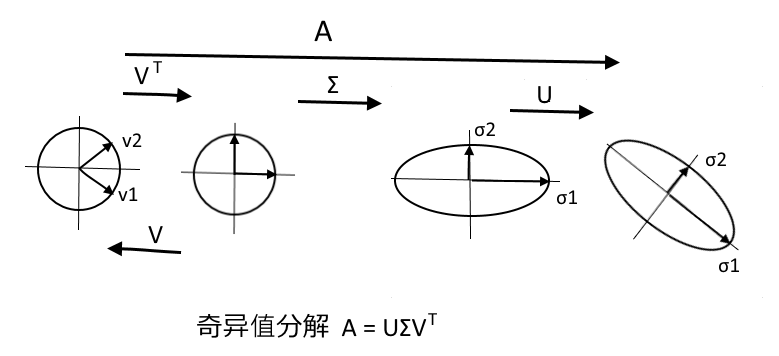
\includegraphics[width=0.7\linewidth]{pic/20450596leeoio001j6199.png}
	\caption{奇异值分解}
	\label{fig:20450596leeoio001j6199}
\end{figure}

\kaishu

奇异值分解(简称SVD)说:对于秩数为r的m*n矩阵A,可以分解成 $ A = U\sum V^T $,这里U是m阶正交阵,V是n阶正交阵,Σ是主对角线上是从大到小的正数$ \sigma_1,\sigma_2, \cdots , \sigma_k $,其余都是0的m*n矩阵。这些正数称为矩阵A的奇异值。

\songti

正交阵V表示一个只包含旋转和翻转的坐标变换,它的列向量表示在X空间中那个相互正交的新坐标轴单位向量。奇异值分解表达出A在这新坐标轴方向上,依次表现出从最大σ1到最小σk的向量长度放大率,直至退化到0的算子作用。U表示在Y空间经过正交变换的新坐标系统,它的前k个列向量作为新坐标轴的单位向量,依此对应着那些经过放大作用后的向量方向。矩阵Σ表达算子这些从最大到最小放大率和秩。

从上述$ AV_i=\sigma_iU_i $关系和正交阵V构造,在$ Ker(A^T) $中选取一组基向量补足列向量,让U矩阵满秩,我们知道不论U是什么都有分解式$ A = U\sum V^T $成立。现在证明U可以是正交阵。$ AA^T = (U\sum V^T)(V\sum^TU^T)  =  U(\sum\sum^T)U^T $,$ AA^T $是对称阵,它可以通过正交变换对角化,而$ \sum\sum^T $是对角阵,其对角线上的元素集合即特征值是由$ AA^T $唯一确定的,这意味着这里的U是那个特征向量组成的正交阵。

如何简单地计算V和放大系数$ \sigma_i $依上面相同的思路,注意到$ (A^TA) $是个半正定的对称方阵,它可对角化,有非负特征根在对角线上。通过解$ (A^TA) $的特征方程,求出特征根和单位特征向量,调整这些单位特征向量在矩阵中排列的顺序,使得对应的特征值从大到小,构造正交阵V,算子的放大系数便是这些特征根的正平方根。细节如下。

记$ Im(A^T) $里的向量$  {V_1,V_2, \cdots,V_k}  $与$ Ker(A)  $里 $ {V_{k+1}, \cdots, V_{n}} $,组成单位正交阵V,设$ AV_i=\sigma_iU_i , i=1, 2, \cdot,k,\sigma_i$是个正数$ ,AV_i=0,i=k+1, \cdots, n $,因为U的列向量也都是单位正交的,所以 有$  V^{-1}(A^TA)  =  (AV)^T(AV)$  $= $  $ U^Tdiag($  $\sigma_1^2,\sigma_2^2, \cdots, \sigma_r^2,0, \cdots,0)U = $   $ diag(\sigma_1^2,\sigma_2^2, \cdots, \sigma_r^2,0, \cdots,0) $,这式子表示正交的坐标变换V,把对称阵$ (A^TA) $变成对角线上是$ (\sigma_1^2,\sigma_2^2, \cdots, \sigma_r^2,0, \cdots,0) $的对角阵。$ (A^TA) $是半正定的对称阵,它的特征值是$ (\sigma_1^2,\sigma_2^2, \cdots, \sigma_r^2,0, \cdots,0) $,从大到小排列,它们对应着V中的列向量为特征向量。这告诉我们,可以通过$ (A^TA) $的特征值和特性向量得到这r个正数$ \sigma $值和单位正交阵V和U,这时有 $ AV = U\sum $,即$ A = U\sum VT $。

注意这个分解中的矩阵U和V有时不是唯一的,在$ i\ge k $时V中的列向量$ V_i $可以在Ker(A)子空间中任选一组正交的基向量,U中的列向量$ U_i $可以在$ Ker(A^T) $子空间中任选一组正交的基向量,当$ A^TA $有重根的特征值时,相应的列向量可以在它们的不变子空间中任选一组标准正交基向量,它们都构成让分解式成立的不同矩阵。但这些的不同都不影响它特征分析和应用。

谱分析在物理和应用数学上有着非常清晰物理含义,对称矩阵总是可以通过坐标的正交变换对角化,这意味着线性空间中的向量可以按不同的维度(频率)分解,可对角化的方阵只是对线性变换的谱分析。奇异值分解是谱分析思想在任意线性算子上的推广。

奇异值分解从子空间分划和坐标系旋转翻转的角度揭示算子的放大特性,这个分解式还未凸显出它最引人注目的用处。将这分解式展开:

\[A = \begin{pmatrix}U_1& \cdots&U_k &\cdots &U_m\end{pmatrix} \begin{pmatrix} \sigma_1 & & & & &0 \\ &\ddots & & & & \\ & &\sigma_k & & & \\ & & &0& & \\ & & & & \ddots & \\0&  & & & &0\end{pmatrix} \begin{pmatrix}V_1^T\\ \vdots \\V_k^T \\ \vdots \\V_n^T \end{pmatrix} = \sum_{i=1}^k \sigma_i U_i V_i^T\]

秩数为r的矩阵通过奇异值分解,把它变成了r个秩数为1的矩阵之和:

\[A=\sigma_1U_1V_1^T +\sigma_2U_2V_2^T+ … +\sigma_rU_rV_r^T\]

当r与m和n相比很小时,这在分析、计算及数据储存上带来很大的方便。因为奇异值是按大小顺序排列的正数,我们甚至可以截取这连加式的前几个作为近似和滤噪。这个性质在图像压缩,信号处理,统计上主成分分析(PCA)和机器学习上都有很好的应用。奇异值分解自从1965年有了计算机上有效的算法后,现在已经成为线性代数应用最广的分解式。

在包含着矩阵运算的计算机语言中,一般都有奇异值分解的函数, 在 MATLAB 和 Octave ,可以用svd函数直接得出矩阵A的分解式 A = USVT中的矩阵:[U, S, V] = svd(A);
	\chapter{重修线性代数9——方程}

线性代数的核心问题是解方程。高斯消去法启示的初等变换,至今仍是解线性方程组和矩阵计算的基础。行列式因研究线性方程组解而被引入,带来矩阵的表示,进而联系起抽象的代数。代数能应用于现实中,在于它具备解方程的有效手段。解方程的算法从空间的角度来看是坐标变换,不仅由此易于得出解的表示,也因此能够看到定性的结果。线性方程的解从理论到算法都有着清晰明确的结果。这导致成功的科学理论系统基本都是线性的。

\subsection{线性方程的定性理论}

从X到Y线性空间抽象的线性算子A,作用在向量$ \bm{x} $,映射得到$ \bm{x} $的像$ \bm{b} $,于是有等式$ A\bm{x}=\bm{b} $。这便是线性方程。这式子可以表示任何线性空间中线性算子的作用,一切线性方程都可以表示成这个等式。从已知的A和$ \bm{b} $,求$ \bm{x} $,是解方程。如果这是微分算子的线性组合在函数空间中的作用,则是线性微分方程;对积分算子则是积分方程;在有限维空间则是代数线性方程组。它们有着共同的性质。

$ A\bm{x}=\bm{0} $,叫做齐次方程,它的解构成Y的一个子空间Ker(A),即零空间。满足$ A\bm{x}=\bm{b} $的等式任何一个向量$ x_0 $叫做特解,通解则是特解与零空间中任何一个向量之和。只有$ \bm{b} $在算子的像空间Im(A)中,解才存在。如果像空间就是Y的全空间,即映射是满的,解总是存在的。当零空间只有一个0向量时,线性方程若有解,则是唯一的。线性空间是无穷维时,上述的结论还涉及到收敛的问题,这要求算子是闭的。巴拿赫空间(定义了距离且柯西列都收敛的向量空间)中,线性算子定义域D(A)中的序列$ (x_n) $,当$ \bm{x}_n\rightarrow \bm{x} ,A\bm{x}_n\rightarrow\bm{b}$,有$ \bm{x} $也在D(A)中,且$ A\bm{x}=\bm{b} $,则称A是\textbf{闭的}。

从代数的角度来看,从Y映射到X的线性算子$ A^R $和$ A^L $,若 $ AA^R= I $ ,称 $ A^R $ 是A的\textbf{右逆};若$ A^LA=I $,称$ A^L $是A的\textbf{左逆}。如果算子有右逆,从$ A(A^R b)= b $得知,至少存在着一个解$ x_0=A^Rb $。如果有左逆,若x是方程的解,因为$ x=A^L(Ax)=A^Lb $,它则是唯一的解。当$ A^L=A^R $时,依定义是A的逆$ A^{-1} $,这时方程的解存在且是唯一的,反之亦然。对此不难有,无穷维的巴拿赫空间(包括了希尔伯特空间)的逆算子定理:一一满映射闭算子的逆存在,而且是有界的。

\subsection{有限维线性方程组}

在有限维线性空间,线性算子表达为矩阵A,可以从空间看到更清晰的图像。

\[\begin{matrix} a_{11}x_1+a_{12}x_2+\cdots+a_{1n}x_n=b_1 \\ a_{21}x_1+a_{22}x_2+\cdots+a_{2n}x_n=b_2 \\ \vdots\\  a_{m1}x_1+a_{m2}x_2+\cdots +a_{mn}x_n=b_m\end{matrix}\]

表示成m*n矩阵形式,用算子和向量的符号把方程简记如下:

\[A=\begin{pmatrix}a_{11}& a_{12}&\cdots& a_{1n} \\ a_{21}& a_{22}&\cdots& a_{2n} \\ \vdots\\ \\a_{m1}& a_{m2} &\cdots& a_{mn}  \end{pmatrix} \textbf{x}= \begin{pmatrix}x_1 \\x_2 \\ \vdots \\x_n \end{pmatrix},  \textbf{b}= \begin{pmatrix}b_1 \\b_2 \\ \vdots \\b_m \end{pmatrix},A\textbf{x}=\textbf{b}\]

从线性算子角度来看,它自然拥有上面抽象线性方程的全部结论。

将矩阵第j列看成是一个列向量,记为$ A_j $,即$ (\bm{A_1}\ \bm{A_2}\  \cdots \  \bm{A_n}) = A $这个线性方程组可以写成:$ x_1\bm{A_1}+x_2\bm{A_2}+\cdots+x_n\bm{A_n}=\bm{b} $

这意味着解是将方程组右边的向量$ \bm{b} $,表示为矩阵中列向量线性组合的系数。算子A的像空间,即是矩阵A的列空间。线性方程组有解的充要条件是:方程组右边的向量是矩阵列向量的线性组合,或说它与它们是线性相关的。齐次方程$ A\bm{x}=\bm{0} $没有非零解,意味着A的列向量是线性无关的。显然,如果非齐次方程有解,方程组右边的向量,是这些线性无关的列向量的线性组合,这个组合的表示是唯一的。如果齐次方程有非零解,线性相关的列向量则有多种的线性组合,表示同一个向量。这对应着这方程组有唯一解或无数的解。

再从空间的几何图像来看。线性方程组的每个方程,例如第i个方程,$ a_{i1}x_1+a_{i2}x_2+\cdots +a_{in}x_n =b_i $ ,将系数看成矩阵行向量\textbf{a}$ _i $的分量,用向量内积的式子记为 $ \left \langle \bm{a_i}, \bm{x} \right \rangle=b_i $ ,这表明满足这第i个方程解x,是空间中一个变动的向量,它与向量$ \bm{a}_i $的内积是$ b_i $,所以满足这第i个方程所有的向量x的所指的点,在n=3时是3维空间中的一个平面,对于一般的n,是n维空间的一个\textbf{超平面}(注:这里的超平面,指n维几何空间中的n-1维平面,它不是指那种过原点作为线性n-1维子空间的超平面),它与向量$ \bm{a}_i $的方向垂直,与原点的距离是 $ b_i/\|\bm{a_i}\| $。

这m个线性方程组的解,是这m个超平面的交集,它是n维空间里的一个子集,在极端情况可以是一个点或空集。也就是说线性方程组可以有无数个解,有唯一的解或无解。

\subsection{解线性方程组}

线性方程具有非常确定的解法和清晰理论结果。这是它能被广泛应用的原因。我们必须充分地了解这些结果,才有把握应用好计算机求解的软件。

中学代数让我们习惯于方程的个数等于未知数的个数,其他情况没有答案。在应用中,我们可能有多于或少于未知数的方程,实际上即使等量的方程数,由于在数学模型中抽象为属性的未知数相关或相近,方程作为实验的样本也可能是线性相关的相近的,这样解方程也可能陷入无解、多解或不确定解的情况。我们需要了解从实用角度怎么处理这些问题,并理解计算软件解方程的函数。下面我们分析n个未知数m个线性方程组$ A\bm{x}=\bm{b} $中,矩阵A的不同情况,然后汇总答案。

\textbf{A是满秩方阵}。这时A的逆A-1存在,方程个数m与未知个数n相等,且列向量线性无关,方程的解可以表示为$ \bm{x}=A^{-1}\bm{b} $.

\textbf{A是列满秩的长方阵}。这是列向量线性无关,方程个数多于未知个数的情况,矩阵A的秩$ r = n \le m $,这时方程可能有解也可能无解。我们不能扔掉几个方程来求解,那犯了丢弃实验数据去修改计算的错误,正确的做法是求误差最小的解y,

\[\min_\textbf{y}\|A\textbf{y}-\textbf{b}\|^2\]

用最小二乘法可以推出正规方程(normal equation)$ A^TA\bm{y}=A^T\bm{b} $,它的解y是满足方程式约束的最小误差向量。在几何直观上,这最小误差解$ \bm{y} $对应着向量b在A列空间投影$ P\bm{b} $的解,即$ A\bm{y} = P\bm{b} $。投影的算子$ P=A (A^TA)^{-1}A^T $. 

对于列满秩的A,方阵$ A^TA $是满秩的,$ A^TA $的逆存在。显然 $ A^L=(A^TA)^{-1}$  $A^T $ 是A的左逆。若方程右边向量\textbf{b}就在A的列空间中,方程有解,这时$ P\bm{b}=\bm{b} $,正规方程的解\textbf{y}也就是原方程的解\textbf{x}。从左逆的存在,知道$ \bm{x}=(A^TA)^{-1}A^T\bm{b} $是唯一的解。

\textbf{A是行满秩的扁方阵}。这是矩阵列向量线性相关,方程个数少于未知个数的情况,矩阵A的秩$ r =m \le n $,这时方程有多个解,解点构成n维空间中一个n-m维的超平面。只要求出一个特解$ \bm{x}_0 $,通解便是$ \bm{x}_0 $加上A零空间的向量。对于这个行满秩的A,方阵$ AA^T $的逆存在,显然$ A^R=A^T(AA^T)^{-1} $是A的右逆,$ \bm{x}_0= A^T(AA^T)^{-1}\bm{b} $是方程的一个特解,若\textbf{z}是A的零空间中的一个向量,它们的内积$ \langle \bm{x}_0, \bm{z}\rangle=\langle A^T(AA^T)^{-1}\bm{b}, z\rangle =\langle(AA^T)^{-1}\bm{b}, A\bm{z}\rangle=\angle(AA^T)^{-1}\bm{b}, 0\rangle= 0 $,这说明$ \bm{x}_0 $与零空间正交。而方程的通解是由$ \bm{x}_0 $与零空间中向量之和,这些端点构成了解平面。$ \bm{x}_0 $与这解平面垂直,$ \bm{x}_0 $的长度是从原点到这解平面的距离,是这方程中长度最短的解。

\textbf{A是秩亏缺的}。这是矩阵列向量线性相关,方程个数多于线性无关的未知个数情况,矩阵A的秩r小于m和n,这方程可能是无解但一旦有解则有多解。这时矩阵A没有左逆或右逆,更不可能有逆。但有一种\textbf{伪逆} ( Moore – Penrosepseudoinverse )可以用来给出它的广义解。让我们看看这是什么?

秩数为r的m*n矩阵A,都可以做奇异值分解 $ A= U\sum V^T $,这里U是m阶正交阵,V是n阶正交阵,$ \sum $是主对角线上有从大到小的r个正数,其余都是0的 $ m*n $ 矩阵。将Σ主对角线上非零元素取倒数,构造n*m矩阵$ \sum + $如下:

\[\Sigma \Sigma^+ = \begin{pmatrix}I&0\\0&0\end{pmatrix}_{m\times m},  \Sigma ^+\Sigma = \begin{pmatrix}I&0\\0&0\end{pmatrix}_{n\times n}\]

令$ A^+=V\sum+U^T $,$ A^+ $称为A的伪逆。从这伪逆的构造中很容易看出它的几何意义:$ AA^+ $是对A的像空间Im(A)投影算子, $ A^+A $是对$ A^T $像空间$ Im(A^T) $的投影算子。不难从几何含义中或从代数式子中推出,它还有这些性质:$ AA^+A=A,A^+AA^+=A^+,(AA^+)^T=AA^+,(A^+A)^T=A^+A $.

这个伪逆$ A^+ $,当A是满秩方阵时等于它的逆$ A^+=A^{-1} $,A是列满秩时等于左逆$ A^+=A^L $,A是行满秩时等于右逆$ A^+=A^R $,所以它是包含了这三种情况广义的逆。

令$ \bm{y}_0=A^+b $,它是方程$ A\bm{y}=AA^+\bm{b} $的解。因为$ AA^+ $是A的像空间投影算子,如果\textbf{b}在A的像空间中,$ y_0 $就是$ A\bm{x}=\bm{b} $方程的一个解,否则它是与之最小误差的解。如果矩阵A的秩小于它的列数,方程的解或最小误差解是多个的。这个$ \bm{y}_0 $是从原点到解平面的垂线。总之$ \bm{y}_0=A^+\bm{b} $,可以作为各种情况下,满足线性方程组约束的最好结果。

上述都是解线性方程组最基本的内容。下面的练习是熟悉、记忆、应用这些知识的最好手段。

\kaishu

在MATLAB或Octave中,通过验证下面的例子来熟悉用计算机的矩阵计算。赋值2x4矩阵 A=[1 2 3 4;2 3 4 5],函数N=null(A)给出A的零空间的一个标准正交基(线性无关向量组),rank(A)给出矩阵A的秩,size(A)给出A的行数和列数。用矩阵乘法A*N,验证N是A的零空间,随机给几个矩阵通过以上指令,来验证秩-零度定理。

在数值计算中的定性结果与允许的误差有关,在一些函数变量中都有允许误差的参数tol,如null(A,tol)和rank(A,tol),不同的误差允许值可能得出不同的结果。设A2=[1 2 3 4;2 3 4 5;2 4 6 8.01]计算tol=0.01和 0.001时,B的秩,零空间。为什么B*N也近似为0矩阵?

在MATLAB和Octave中用于计算矩阵A的逆的指令函数是:inv(A),计算伪逆是:pinv(A).建议读者在计算软件中,用几种2x3和3x2行满秩、列满秩,秩亏缺的矩阵A及相应的b向量,运用矩阵的乘法和这些函数,计算左逆,右逆,伪逆,投影算子,方程解并验证它们间的关系。

可以用x=Ab来得到线性方程组A*x=b的一个解,它等于pinv(A)*b. 验证x与Null(A)中任何向量的和,都是这线性方程组的解。

\songti

\subsection{微分方程}

微分方程与代数方程的区别,在于前者算子作用的线性空间是无穷维,后者则是有限维的。微分和积分都是线性算子,微积分的计算基本都是映射和线性代数运算,只因涉及有无穷个线性无关的向量,则要考虑无穷个线性组合的收敛问题。有这个理解在心,就不至迷惑于在线性代数中未见的许多条件,放心从抽象的高度,透视许多繁杂的定理和计算方法。

在计算机时代之前,人们用函数族作为无穷维线性空间的基,用级数或积分来表示解与系数中的函数,在算子作用下将微分方程变成代数方程来求解。这在物理研究中被广泛地采用。

另一种解法是对无穷维线性空间进行线性变换,如拉普拉斯变换,将解微分方程变成在另一个线性空间中的代数运算。在现代控制理论中,对线性动态系统的微分方程,应用这种解法,已成为分析和计算的必备的数学工具。

在计算机时代,机器可以直接给出数值解。应用者不必像旧时代那样,花费大量时间学习各种计算方法和技巧了。只需要有一些基本的概念。

高阶常微分方程,通过定义导数变量$ x_{k+1}(t)=x'_k(t) $的方式,把它写成一阶微分方程的向量形式$ x'(t) = \bm{f}(\bm{x}, t), \bm{x}(0) = \bm{c} $. 将方程两边积分后,有定理证明只要这个$ \bm{f} $“足够光滑”(满足Lipschitz条件),微分方程存在着唯一的解,整理成线性算子作用的形式是:$ \bm{x}(t) =\phi(x,t)\bm{x}(0) $. 对于一个离散的时间序列,可以写成递推的式子,如龙格-库塔法,来计算这些向量值。

离散的数值计算作为精确解的近似是否有意义,取决于它对初值和参数变化的稳定性。对于线性常微分方程,这个稳定性可以通过对微分方程矩阵的特征值分析容易得知。这在现代控制理论中的课程中有详细介绍。
	\chapter{重修线性代数10——计算}

线性代数源于解线性方程组,这是数学公式逆向的计算。在计算机时代之前,限于手工计算的能力,线性代数多是作为理论研究的基础。到了现代,它已是理工科但凡涉及到统计和数值计算必备的工具了,最近更成为机器学习热门的基础课。

\section{病态系统}

数学的理论无论多么漂亮,应用到实践,总要落实到数值的计算。线性系统是最简单实用的数学模型,理论上解线性方程组有非常确定的结果,但也可能有意外。让我们看一个例子。

\kaishu

解线性方程组0.410x + 0.492y = 0.902,0.492x + 0.590y =1.082;得x=1,y=1. 若第一个方程右边的0.902略有变动成为0.901,解就变成x= 4.5976,y= -2.000; 同样第二个方程右边的1.082的数值变成1.081后,解就变成x= -2.000,y= 3.500.

\songti

实践中的数据总有些误差,方程的参数微小的变动,竟让计算结果面目全非,这确实让人始料不及。这样不稳定的计算结果在应用上毫无价值。问题在于,这个差异并非是计算误差造成的,将它们代入方程验证都精确无误. 这就无从计算上来改善了。这种对参数微小变动敏感的系统称为是病态的(ill-conditioned),这是数学模型的问题。这个例子,在几何图像上不难看到原因。每个方程在空间确定一条直线,方程的解是这两条直线的交点。这两个方程确定的直线近于平行,所以位置略有变化(红线和绿线),它们的交点(红点和绿点)的位置就差得很远。

% TODO: \usepackage{graphicx} required
\begin{figure}[h]
	\centering
	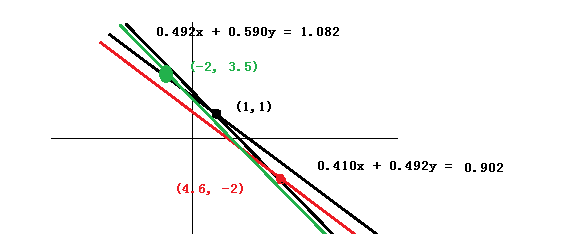
\includegraphics[width=0.7\linewidth]{pic/1612386nrnueyrye6k8kq4.png}
	\caption{一个病态系统的例子}
	\label{fig:1612386nrnueyrye6k8kq4}
\end{figure}

在数值分析中,条件数(conditionnumber)用来描述数学模型系统的微扰对计算结果的影响。大致说来,对条件数κ,$ log_{10}κ $是你在计算可能要丢掉的数字位数$ (log_{10}\|Δx/x\|\leq log_{10}κ+ log_{10}\|\delta b/b\|) $,当然这个数κ是很难确定的,它是作为相对误差上界的估算。对于解线性方程组 Ax=b,它的意思是$ \|\delta x/x\| \leq κ\|\delta b/b\| $,经过推导有$ κ(A) =\|A\|*\|A^{-1}\| $,对通常的$ L_{2} $范数$ κ(A)= |\sigma_{max} /\sigma_{min}| $,它是A做奇异值分解后最大与最小奇异值之比,在可对角化的矩阵即是最大绝对值的特征值与最小绝对值的特征值之比。正交阵(或酉阵)的条件数是1,这是最小的矩阵条件数值,所以正交阵具有最好的计算稳定性。这说明我们建立线性的数学模型时,要尽量选择近于正交的数据来建立方程组。

在MATLAB或Octave可以用cond(A)指令计算A的条件数。上面例子中κ(A) = 6099.6.

\section{支点对计算的影响}

高斯消去法几乎是线性代数各种计算的基本手段。它不仅用来化简矩阵计算行列式。对线性方程组的求解,把方程右边的列向量拼入左边的矩阵,成为增广矩阵(A,\textbf{b}),然后对它进行行间的变换,直至左上角部分变成三角阵,然后对照右边最后一列,判断方程是否无解,若有解则用右边三角阵部分迭代求解,多解时则同样可以迭代解出零空间的线性无关向量。

矩阵求逆,则把单位阵拼入左边成为增广矩阵(A,I),右边部分记录了所有的行变换,与解方程一样,先从上到下,用支点(pivot)即主对角线上的元素,消去对角线下非零元素,把左边部分变成上三角阵。然后从下到上消去对角线上非零元素。如果A是满秩的,增广阵终将成为$ (I, A^{-1}) $,右边即是逆矩阵。在这从上到下,三角阵化的消去过程中,只要支点是非零的,我们不需要交换行来进行,这时增广矩阵的右边的子矩阵是个下三角矩阵U,而左边是个上三角的子矩阵L,这时的增广矩阵(U,L)实现了LU分解。

理论上,只要这个过程中的支点是非零元,用消去法解方程、求逆和做LU分解都是可以的。实际上仍然会遇到问题。看下面用第一行消去第二行第一列,做的LU分解。

\[A=\begin{bmatrix} 0.0001&1\\ 1&1 \end{bmatrix}=\begin{bmatrix} 1&0\\ 10,000&1 \end{bmatrix}\begin{bmatrix} 0.0001&1\\ 0&-9999 \end{bmatrix}=LU\]

条件数κ(A)=2.6184尚属于良态,而$ κ(L) =10^{8},κ(U) =0.9999*10^{8} $,都是非常病态了,用这个分解做计算会带来很大的误差。问题在于计算过程中支点的数值太小,解决的办法是运用支点做消去法前,先搜寻支点所在位置及下面,从中选出最大元,交换这两行使得最大元在支点位置。对这个矩阵A,是先交换上下两行,然后再做消去法,这样有:

\[P=\begin{bmatrix} 0&1\\1&0\end{bmatrix},\;PA=\begin{bmatrix} 1&1\\0.0001&1 \end{bmatrix}=\begin{bmatrix}1&0\\0.0001&1\end{bmatrix}\begin{bmatrix} 1&1\\ 0&0.9999 \end{bmatrix}=LU\]

这时κ(L) =1.0001,κ(U) =2.6182,都是良态的。所以在矩阵的计算中,为了减少误差经常需要交换行或列,这个步骤可能隐含在算法中,也可能需要表示在计算机函数的式子里。通常用置换矩阵P来表示这些行或列的交换,如在MATLAB或Octave中指令 [L U P]=lu(A),指的是 PA = LU的分解。为了减少误差,分解指令[G U]=lu(A),如果需要交换行,则把P吸收在G中,$ G=P^{T}L,A=GU $,这时G不再能保持L的下三角阵的形式了。

\section{机器学习}

人们走向理性,依赖于在意识层次上的逻辑求证。不明因果机理的预测和难以追踪判断过程的结论,都被视为迷信而被科学排斥。算术曾经是解决实际问题计算唯一可靠的途径,在那里应用问题分门别类地归纳成不同的类型,诸如鸡兔同笼、宝塔装灯等等,每个计算步骤和所得的数量,都有直观可以理解的含义。代数的方法偏离了直观推理的途径走向抽象,三个未知数的线性代数方程,已经难以用单向逻辑推理的路径来追踪它解法的含义。我们只能用严格的逻辑,来证明每一步的代数运算都是等价或蕴含原来问题的不同描述。由此,我们可以用简化了问题的计算答案来回答原来的问题。在理性求证的过程中,我们把解方程的代数方法看成可以信赖的中间站,将现实问题的各种关系表示成方程后,放弃了对解法计算的每一步的追踪判断,直接承认它的结果。物理等科学研究沿用这种思想,把实际问题描述成数学模型后,直接依赖于数学的分析和计算。

机器学习将代数方法的启示推向另一个高度。它不再依赖于人力把实践中的预测和判断问题描述成一个数学模型,而是运用一个带有众多可调参数的通用数学模型,直接利用拥有的数据来调节参数自行寻找适用于这一类数据的具体模型,以此应用解答预测和判断问题。

与代数的方法取代算术方法的困惑一样,机器学习的调整模型参数及应用模型的计算机制,在数学上都是精确有效的。但巨大数量的可变参数,难以把这简单数学模型的一个具体的辨识判断过程,解析成为像物理规律那样单纯过程的因果性机制,无法用简单逻辑推演的跟踪来获得理解。机器学习的智能渐渐走离我们理性的监督,却成为未来应用计算的利器。下面简单对此作介绍。

机器学习与人类经验公式和分类的基本计算是一样的,都是用线性的方法计算参数,找出与实验数据匹配最小误差的数学模型,以此用来预测未知。对经验公式,用的是线性回归,找出那个线性函数,它是个与实验数据误差最小的的超平面;对模式识别的分类,用逻辑回归,找出那个判别函数,它是个分隔两类样本的超平面,与实验数据的误差最小。最后它们都归结为确定那个超平面的线性代数计算。(注:这里的超平面,指n维几何空间中的n-1维平面,它不是指那种过原点作为n-1维线性子空间的超平面。)

在n维线性空间中,满足内积$\langle \mathbf{z},\mathbf{a}\rangle = b $的向量\textbf{z},构成n维几何空间中的一个n-1维平面,将向量扩充到n+1维空间,令$ \mathbf{x}=(1,\mathbf{z}^T)^T, w=(-b,\mathbf{a}^T)^T $,这个内积可以表示为$ \langle \mathbf{x},\mathbf{w}\rangle= 0 $.

\begin{figure}[t]
	\centering
	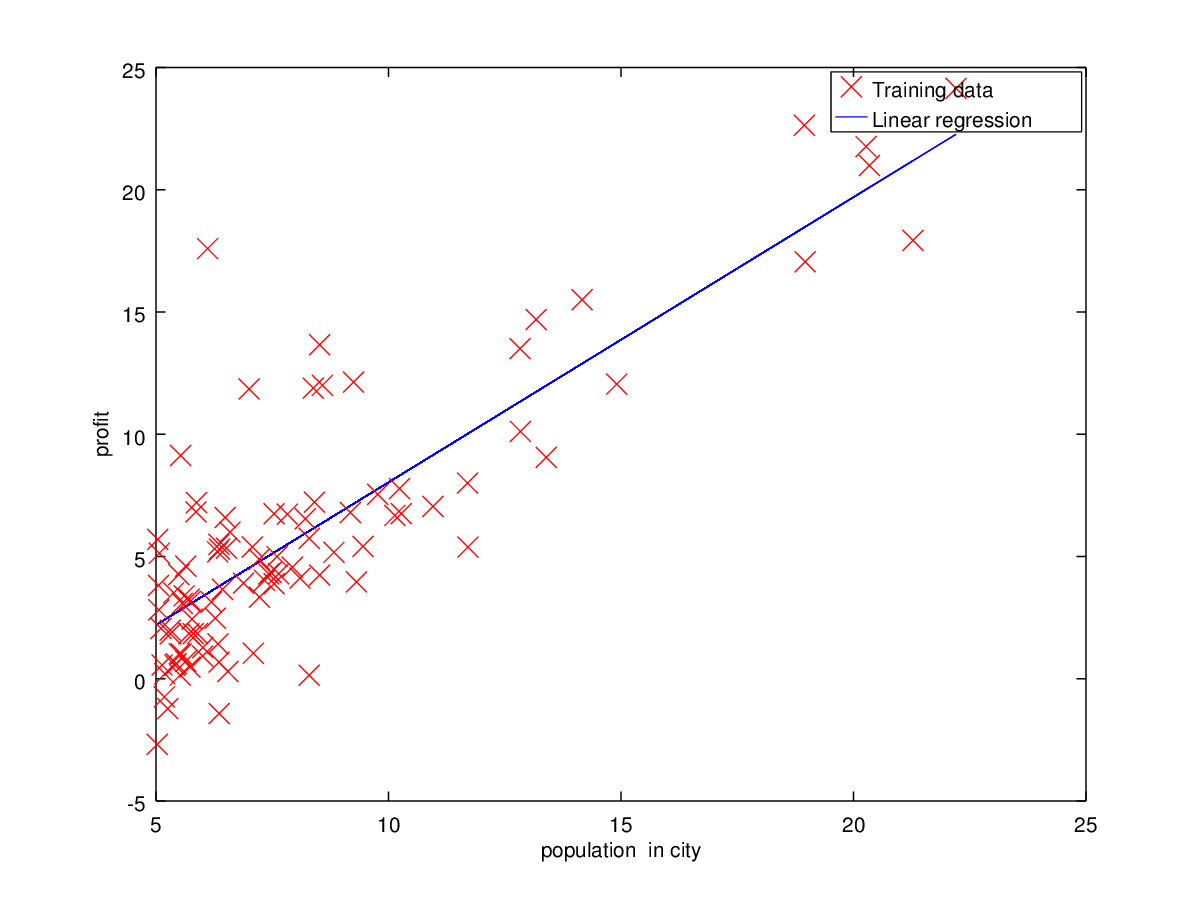
\includegraphics[width=0.49\linewidth]{pic/161238petg2epyqhslbulz.png}
	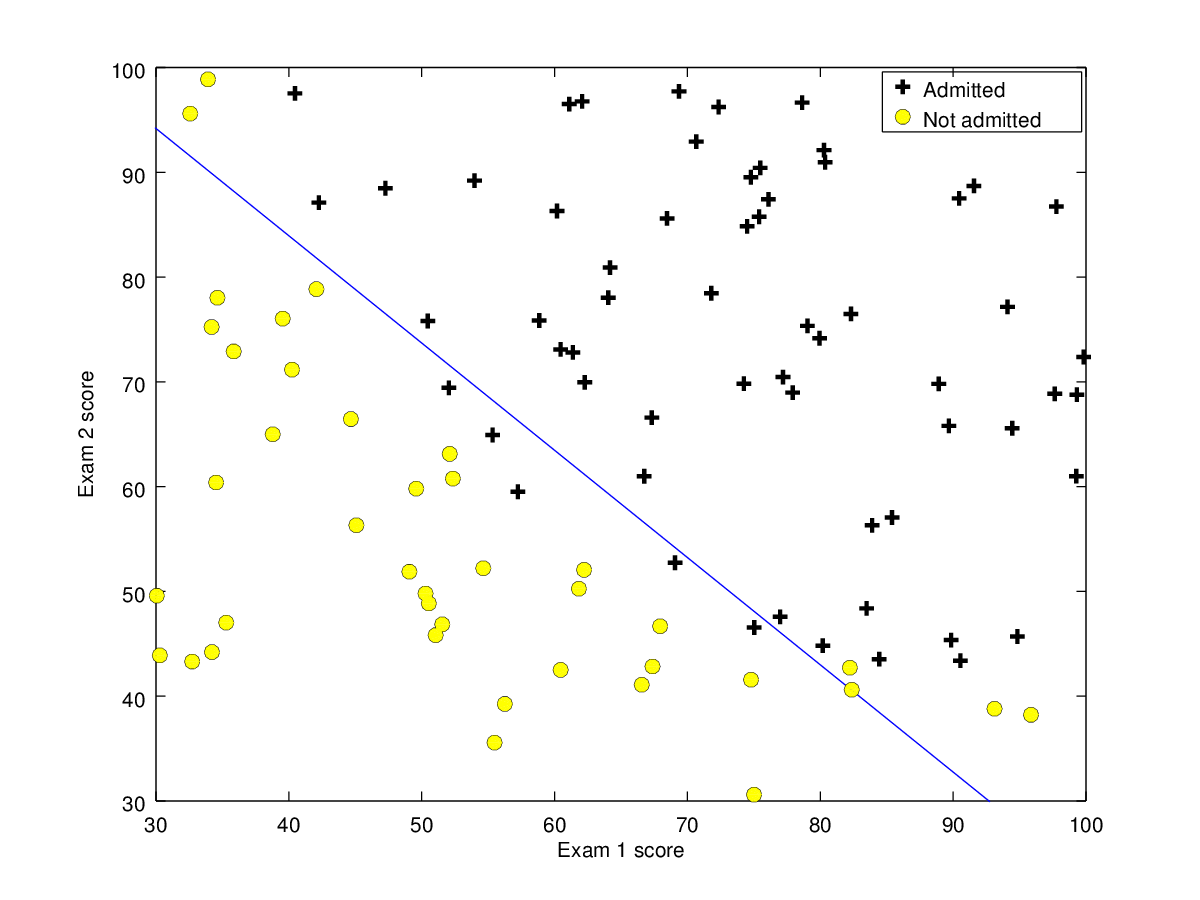
\includegraphics[width=0.49\linewidth]{pic/161239i3870x2cvwmclc09.png}
	\caption{线性回归}
	\label{fig:161238petg2epyqhslbulz}
\end{figure}

\textbf{线性回归(linear regression)}:在线性回归的数学模型中,假定有足够多描述事物的属性,表示为函数的变量,归纳了经验的数值公式是这些属性变量的线性函数,我们尽可能应用大量的实验数据,来统计出误差最小的模型的系数。具体计算如下。

假设n维的属性向量$ \mathbf{x}_{i} $和公式结果标量$ y_{i} $,经验公式有线性的关系$ \langle \mathbf{x}_i, \mathbf{w}\rangle = y_{i}$,其中w是待定的参数向量。我们有m组实验数据,m >> n,希望对所有的实验数据 $langle \mathbf{x}_i, \mathbf{w}\rangle$ 都非常靠近 $  y_i $ . 在上一篇中提到,这是列满秩矩阵解线性方程组的问题,可以用最小二乘法求解。

把m个n维行向量$ \mathbf{x}_i^T $写成m*n矩阵X,m个$ y_i $列成向量y。设误差函数$ J(\mathbf{w}) =1/2\|X\mathbf{w} - \mathbf{y}\|^2 = (X\mathbf{w} - \mathbf{y})^T (X\mathbf{w} - \mathbf{y})/2 $,计算问题是,求让$ J(\mathbf{w}) = (X\mathbf{w} - \mathbf{y})^T (X\mathbf{w} - \mathbf{y})/2 $取最小值的向量$ \mathbf{w_0} $.  

$ J(\mathbf{w})  $是个在n维空间中的二阶幂函数的曲面,它有唯一的极小值在梯度为零处,即梯度$ X^T ((X\mathbf{w} - \mathbf{y}) = 0 $,这可以表示成正规方程$ X^TX\mathbf{w} =X^T\mathbf{y} $. 它有唯一解$ \mathbf{w_0} =(X^TX)^{-1}X^T\mathbf{y} $.  在大数据的情况下,这个公式解的计算量太大,我们可以采用迭代的方式求解,这通常从任何一个w的初值开始,沿着这个梯度$ X^T ( X\mathbf{w} – \mathbf{y}) $下降的方向,迭代逼近这个极值点$ \mathbf{w_0} $.

\textbf{逻辑回归(logistic regression)}:模式识别是进行逻辑分类,它假定在足够多属性为坐标的多维空间中,用一个超平面把空间分成两半,分别对应着不同的逻辑值。逻辑回归用来确定这个将实验样本中分类误差最小的超平面。

在n维线性空间中,满足内积 $ \langle \mathbf{z}, \mathbf{a}\rangle = b $的向量\textbf{x},在\textbf{a}方向上投影的长度都是$ b/\|a\| $,这些x向量的端点构成的n-1维的平面,这超平面与原点的距离是$ b/\|a\| $。空间上面的点依指向它的向量\textbf{z}在\textbf{a}上面的投影被这超平面分成两个部分,依内积$ \langle \mathbf{z}, \mathbf{a}\rangle  $是否大于b,确定它们属于哪一类。这是模式辨识和机器学习中分类最为基本的直观图像。

采用上面扩充向量的符号,这个超平面是由\textbf{w}的数值来确定的,所谓的学习是用样本的数据$ \mathbf{x}_i $和对应的0或1的分类值$ y_i $,来计算这个\textbf{w}。数学模型的预测值是由判断函数$ g(\langle x,w \rangle ) $来确定,理论上$ g(\langle x,w \rangle )= (sign(\langle x,w \rangle)+1)/2 $,但为了便于计算梯度,多数取sigmoid 函数g(t)=1/(1+exp(-t)).

我们同样用求误差函数$ J(\mathbf{w}) =1/2\|g(X\mathbf{w}) - \mathbf{y}\|^2 = (g( X\mathbf{w}) –\mathbf{y})T (g( X\mathbf{w}) –$   $\mathbf{y})/2 $ 最小的方法,来得到极值点$ \mathbf{w_0} $,用迭代的方法沿着梯度下降的方向,逼近这个极值点$ \mathbf{w_0} $.

\section{世界是线性的吗?}

上一节说,机器学习的核心算法线性回归和逻辑回归,应用的都是线性模型。这也是经验公式和模式识别的基础。我们的世界都是线性的吗?

开篇时也说,令人感到幸运和疑惑的是,科学研究上凡是用到数学,有着漂亮定性和定量结果的,基本上可以变成一类线性系统,或者用它来逼近。为什么?

世界是线性的吗?其实不是,只是非线性的系统正向计算不难,但难以反向求解,更无法分部综合。我们能用数学工具取得很好结果的,基本上是线性系统。力学是线性动态系统,绝大多数电路是线性系统;描述连续介质,能量和场的波动,传导,稳定状态的数理方程是线性系统。非线性系统可以用两种方法将它应用线性系统的方法来处理。一是可以在足够小误差的邻域看成是线性的;微分几何用曲面上点的邻域,投影到与之相切的线性空间来计算;非线性动态系统控制稳定或跟踪已知轨迹时,可以用线性系统来近似。二是在应用上尽可能把系统处理成线性的,而把非线性部分局限在一小处或作为输入,以便分析和综合。难以照此办理的许多非线性系统即使有精确简单的方程描述,如混沌系统、联结主义模型,无论在定量和定性上,都难以深入。科学和技术与一切在竞争博弈中的发展一样,都是路径依赖的。某一方向取得突破,人们蜂拥而至,用先创的概念作为后建的基石,建构我们理解的世界。科学发展至今,解释事物的理论无所不在,我们似乎已经充分了解了这个世界,其实这不过是看见在科学这条高速公路旁的城镇,公路不可达之处是不可知的荒野。但是无论如何,线性代数已是现代科学知识的基础构件,我们必须能在头脑中想象它。

机器学习的线性模型怎么用在这个并非是线性的世界?线性回归怎么拟合一条曲线上的数据?怎么用一个超平面分划由一个曲面界定的类别?答案在于增加维数。空间中任意的样本点集,都可以看作是高维空间中点集的投影,它们可以在高维空间的一个超平面上,或被一个超平面分类。

例如,实验数据(1,4), (2, 9), (3, 20), (4, 37), (5, 60) 是二维空间的曲线 $ y = 3x^2 – 4x + 5 $上的点,在实验中增加一个属性$ x_2 = x_1^2 $的测量,上面的样本点便成为(1,1, 4), (2, 4, 9), (3, 9, 20), (4, 16, 37), (5, 25, 60) 它们在三维空间$ y =3x_2 – 4x_1 + 5 $ 的平面上。增加几个非线性函数作为新的属性,任何曲面都可以用这些具有新属性变量的线性函数来近似。模式识别中的超平面分类也是如此。这样的处理早已在科研和工程上广泛地应用,它类比于将非线性部分局限在一些部件中,在工程上把系统仍然作为一个线性系统来分析和综合。

\section{结语}

现代公理化的数学,要求尽量抽象,从基本定义出发,不借助任何具象,纯粹形式推理来得到结论。这是严谨化确认的要求,但这不是理解、记忆和运用之道。人脑是按联想方式工作的,不能下意识地推及逻辑之远。我们对世界的理解是用象征符号,在头脑中构建的想象。所谓的课程学习是通过语言,将别人的想象串行地传递给自己,在头脑中重构自己的想象。严格数学的训练沿用形式逻辑推理,只能保证这个传递没有形式上的误差,并不能保证能够建构相同的想象。没有想象就难以记忆和应用。所以学数学就像学剑一样,必须首先心中有剑,从概念的定义开始就要有符合这语义的具象,然后沿着定理推论的展开,逐步剔除不合适的想象,构建符合逻辑的图像。学习中的理解是将语言能指的符号串,与所指的想象对应的过程。形式推理永远不能触及所指的内容,所以形式推理的机器没有理解力。能够产生理解和灵感的,是在头脑的想象世界中看到的内容。这需要拥有丰富的具体实例的素材才能构建。因此学习数学只记忆定义、证明和定理不能走远,也没有透视现象的直觉。严谨的数学证明当然很重要,但那只是用来一维地传递信息,和在逻辑上证实想象的真实性的必要手段。把握数学内容的,是能在想象中出现的图像。练习和应用是学好一门课的不二途径。
\end{document}